\documentclass[12pt,fleqn]{article}
\usepackage{amsmath,amsfonts,amssymb,amsthm}
\usepackage{latexsym}
\usepackage{mdwlist}
\usepackage{a4wide}
\usepackage{ae,aecompl}
\usepackage{titlesec}
\usepackage{graphicx}
\usepackage{epstopdf}
\usepackage[singlelinecheck=false]{caption}
\usepackage[round]{natbib}
\usepackage{url}
\usepackage{pdfpages}
\usepackage{subfig}
%\usepackage{subfloat}
\usepackage{hyperref}
\usepackage{setspace}
\usepackage{xcolor}

\usepackage{tabularx, multirow, booktabs}
\newcolumntype{Y}{>{\centering\arraybackslash}X}
\renewcommand{\tabularxcolumn}[1]{b{#1}}

\hypersetup{
    colorlinks,
    linkcolor={red!50!black},
    citecolor={blue!50!black},
    urlcolor={blue!80!black}
}

\newtheorem{theorem}{Theorem}
\newtheorem{definition}{Definition}
\newtheorem{lemma}{Lemma}
\newtheorem{proposition}{Proposition}
\newtheorem{corollary}{Corollary}
\newtheorem{example}{Example}
\newtheorem{remark}{Remark}

\newcommand{\Xomit}[1]{}
\renewcommand{\baselinestretch}{1.1}

\renewcommand{\rmdefault}{ptm}
\titleformat*{\section}{\large\bfseries}
\titleformat*{\subsection}{\normalsize\bfseries}




\begin{document}

\title{\textbf{Dynamic Refugee Matching}\footnote{The authors are grateful to Atila Abdulkadiro\u{g}lu, Daniel Halvarsson, Fuhito Kojima, Johan Grip, John Hatfield, Jean-Jacques Herings, Thayer Morill, Umut Dur, Utku \"{U}nver and Yeon-Koo Che as well as seminar audiences at North Carolina State University, the Ratio Institute (Stockholm), the Swedish Finance Ministry, Vanderbilt University, and the 2018 SAET conference (Taipei) for detailed comments and remarks. Andersson gratefully acknowledges financial support from the Jan Wallander and Tom Hedelius Foundation (P2016-126:1) and the Ragnar S\"oderbergs Foundation (E8/13). Ehlers is grateful to SSHRC (Canada) and FRQSC (Qu\'{e}bec) for financial support.}}

\author{Tommy~Andersson\footnote{Department of Economics, Lund University, P.O. Box 7082, SE--222 07 Lund, Sweden. E-mail: \texttt{tommy.andersson@nek.lu.se}.}, Lars Ehlers\footnote{D\'epartement de Sciences \'Economiques and CIREQ, Universit\'e de Montr\'eal, C.P. 6128, Succursale Centre--Ville, Montr\'eal, Qu\'ebec H3C
3J7, Canada. E-mail: \texttt{lars.ehlers@umontreal.ca}.}\space\space and Alessandro Martinello\footnote{Department of Economics, Lund University, P.O. Box 7082, SE--222 07 Lund, Sweden. E-mail: \texttt{alessandro.martinello@nek.lu.se}.}}

\date{\small{First version: March 27, 2018. This version: \today.}}

\maketitle
\vspace*{-4mm}
\begin{abstract}
\noindent Asylum seekers are often assigned to localities upon arrival using uninformed matching systems, leading to inefficient and unfair allocations. This paper proposes an informed dynamic mechanism as an intuitive and easy-to-implement alternative. This mechanism can be adopted in any dynamic refugee matching problem given locality-specific quotas and that asylum seekers map into specific categories. Any matching selected by the proposed mechanism is Pareto efficient, and envy between localities is bounded by a single asylum seeker. Our simulations show that the proposed mechanism outperforms uninformed mechanisms even in presence of severe misclassification error in the estimation of asylum seeker categories.

\medskip

\noindent\emph{Keywords}: forced migration, market design, refugee matching, dynamics, envy, efficiency.

\medskip

\noindent\emph{JEL Classification}: C71, C78, D71, D78, F22.

\end{abstract}

% REFUGEE PREFERENSER. Discuss. Conclusions?
% Kolla nummer i "RATIO rapport"
% Lägg till Alessandros Appendix

\section{Introduction}
According to UNHCR, 17.2 million persons obtained refugee status in 2016.\footnote{Unless stated differently, all figures in this section appear at \texttt{www.unhcr.org/figures-at-a-glance.html}.} In an attempt to reduce pressure on countries sheltering large numbers of refugees, several international resettlement programs---the largest of which is operated by UNHCR---transfer a selected portion of refugees to countries that have agreed to admit them, and to ultimately grant them permanent settlement.\footnote{In recent years, the United States has been the world's top resettlement country followed, by Canada, Australia and the Nordic countries. Since 2015, the European Union has also organized a series of resettlement programs in an attempt to reduce pressure on the countries located at the external border of the European Union (Greece, Hungary and Italy in particular).} Although in practice these programs rarely take the characteristics and preferences of refugees and receiving countries into account, \citet{bib:JonesTeytelboym2016b,bib:JonesTeytelboym2016a} note that these types of resettlement schemes share many fundamental properties with classical two-sided matching markets with capacity constraints like the school choice problem \citep{bib:AbdulkadirougluSonmez}. Even if the computational and modeling complexity of asylum seeker allocation is higher than that of a typical two-sided matching problem,\footnote{For example, refugees vary in several dimensions (education, spoken languages, household composition, need for healthcare, etc.), which introduce multidimensional constraints and potential complementarities to the matching problem. Complementarities have been studied in matching markets by, e.g., \citet{bib:HatfieldKominers}, \citet{bib:PathakRoth}, \citet{bib:Pycia} and \citet{bib:RothPeranson}.} results from the rapidly growing market design literature can lead to vast improvements in efficiency, equity and feasibility of refugee resettlement programs \citep{bib:Andersson,bib:BansakEtAl,bib:DelacretazEtAl2016,bib:JonesTeytelboym2016b, bib:JonesTeytelboym2016a}.

A crucial similarity between classical two-sided matching problems and refugee resettlement programs is that all available information on both sides of the market---asylum seekers and localities---is known when making the matching. Only once the full set of asylum seekers, their characteristics, and all preferences are known, the matching can take place. However, gathering such information necessarily requires holding asylum seekers in asylum centres for an undefined period of time. Moreover, less than 1 percent of all asylum seekers are part of resettlement programs.\footnote{The UNHCR program, for example, contained files of only 163,200 asylum seekers for consideration by resettlement countries, and of these, only 126,200 actually departed to resettlement countries. Similarly, while more than 2.5 millions people applied for asylum in 2015 and 2016 alone in the European Union, the total number of relocations within the European Union program stands at 24,676 as of July 24, 2017 (European Commission, Press release, 26 July 2017, Brussels).} The vast majority of asylum seekers arrive directly to their host country, where the assignment to localities needs to take place in a short period of time, and without any information on future arrivals. The difficulty of predicting the characteristics of asylum seekers arriving in the near future necessarily introduces dynamics to the problem, i.e., asylum seekers must be assigned to localities directly upon arrival before the identity and characteristics of future arrivals are revealed.
%To the best of our knowledge, such dynamic refugee matching problem has not been studied in the market design literature before.

This paper solves this dynamic refugee matching problem by proposing an intuitive, easy-to-implement and computationally efficient dynamic refugee matching mechanism that, by exploiting refugee-specific characteristics affecting the probability of successful integration at each locality, guarantees an efficient and unenvious matching at each arrival among localities that have not filled their quotas yet. The efficiency and the envy concepts are based on dynamic versions of Pareto efficiency and envy-by-one \citep{bib:Budish}, respectively.\footnote{The importance of these specific properties has also been stressed in several meetings that the authors of this paper have had with the Swedish Migration Board. In fact, in a recent report \citep[Swedish Government,][]{SOU2018}, the Swedish Migration Board is recommended to further investigate the feasibility of some of the ideas presented in this paper.} Despite its simplicity, the proposed mechanism strongly outperforms uninformed mechanisms such as those currently in use in, e.g., Sweden, Switzerland and the United States. Using aggregate data from Sweden and the United States to calibrate random flows of asylum seekers, this paper shows that even if the probability of successful integration for each asylum seeker and locality is unknown and needs to be empirically estimated \citep[as in][]{bib:BansakEtAl}, the proposed matching mechanism increases efficiency by up to 50 percent, and guarantees a reduction in envy of between 7 and 45 percent.

Although the results presented in this paper are not specific to a particular country, Sweden represents a good example for describing the dynamic problem of matching asylum seekers to localities within a country. An asylum seeker who enters Sweden is temporarily placed at a Migration Board accommodation facility in anticipation of either a deportation order or a permanent residence permit. This facility is located in some locality and the problem for the Migration Board can, therefore, equivalently be described as a problem of matching asylum seekers to localities.\footnote{Note that an asylum seeker may be transferred to a different locality once granted a residence permit. However, as the authors of this paper has discussed with the Swedish Migration Board, asylum seekers will ideally stay in the same locality as this creates incentives for the locality to start integrating the asylum seekers immediately after arrival to Sweden. This is, in particular, true for asylum seekers that are classified to belong to ``Track 1'' (Swedish ``Sp\aa r 1'') according to the Migration Board classification systems. These are the asylum seekers that will be granted asylum with a probability close to 100 percent, e.g., because they come from a specific conflict region.} In the process of matching asylum seekers to localities, asylum seekers can be mapped into specific groups, or categories (e.g., based on age, education, language knowledge, etc.). Asylum seekers belonging to different categories not only have different probabilities to integrate overall, but also exhibit particular synergies with specific localities \citep{bib:BansakEtAl}.\footnote{That nationality matters for assimilation has previously been established by, e.g., \citet{bib:RanEtAl}. \citet{bib:EdinEtAl} and \citet{bib:Damm} show that matches between one's nationality and that of other immigrants in a locality affects the probability of successful integration. If one proxies integration with employment,  locality-specific heterogeneities in integration are also evident from aggregate data. 38.1 percent of all asylum seekers with more than 9 years schooling arriving in Sweden in 2014 had an employment at the end of 2016. However, employment probability in this group varies by gender (45.3 percent for males and 25.8 percent for females), and these numbers vary between Swedish municipalities. See the web page of Statistics Sweden (\texttt{www.scb.se}).}

The current Swedish system to dynamically match asylum seekers to municipalities is approximately based on a random assignment coupled with municipality specific quotas. As described by \citet[][p.325]{bib:BansakEtAl}, a similar mechanism is employed by the resettlement offices in the United States and by the federal government in Switzerland. Random mechanisms are uninformed and, consequently, cannot exploit the heterogeneity among localities and asylum seekers to achieve efficiency and fairness. In fact, if such heterogeneity is not taken into consideration, the resulting matching may be both inefficient and unfair (this point is illustrated in Section \ref{SEC:Fair_Efficient}). In contrast to the random mechanism, the dynamic refugee matching mechanism proposed in this paper takes both locality-specific characteristics and the background of the asylum seekers into consideration and, consequently, exploits the heterogeneity among localities and asylum seekers to achieve efficient and fair assignments. The employed efficiency and the fairness concepts are dynamic versions of Pareto efficiency and an extended version of the concept of envy-by-one \citep{bib:Budish}. The latter property means that whenever some locality envies the matching of some other locality, envy can be ``eliminated'' by removing a single asylum seeker either from the matching of envious locality or from the matching of the envied locality.

Envy between localities occurs whenever different categories of asylum seekers are ``demanded'' at different rates among localities \citep{bib:BansakEtAl}. Conflicts between localities arise if an asylum seeker is either in high demand or not demanded at all. In such cases, there must be some rule that determines which locality the asylum seeker should be matched to. This paper resolves such conflicts by means of priority and rejection orders, where the former determines the matching of highly demanded asylum seekers and the latter determines the matching of non-demanded asylum seekers. These orders constitute the backbone in the considered dynamic mechanism that matches asylum seekers to localities. The main theoretical result demonstrates that if asylum seekers are matched to localities based on the proposed mechanism, any matching of asylum seekers at any point in time is Pareto efficient, and envy is bounded by a single asylum seeker (Theorem \ref{THEOREM:envy_efficiency}).

The theoretical results presented in this paper depend on the assumption that localities can perfectly classify asylum seekers as either acceptable or unacceptable. However, even if refugee characteristics are known, such classification will have to be empirically estimated and will, therefore, suffer from misclassification error. To investigate the consequences of such error, this paper simulates and evaluates the performance of the proposed matching mechanism in specific settings calibrated to resemble the United States and the Swedish situations. These simulations show that the proposed matching mechanism outperforms uninformed mechanisms even in presence of severe misclassification error.

At least two properties make our framework different from traditional matching models. First, the sequential arrival of asylum seekers introduces dynamics. Even if dynamic problems have been considered in the literature before, e.g., in a kidney exchange \citep{bib:Unver}, kindergarten allocation \citep{bib:KennesEtAl2014}, daycare assignment \citep{bib:KennesEtAl2014}, and house allocation \citep{bib:BlochCantala,bib:Kurino}, a vast majority of the papers in the matching literature focus on static matching.\footnote{There is also a small literature on dynamic notions of stability, e.g., \citet{bib:DamianoLam}, \citet{bib:Gudmundsson}, \citet{bib:KadamEtAl2018b}, and \citet{bib:Kurino}. See also Section \ref{SEC:literature}.} In static settings, the set of agents, preferences, etc. are known when solving the matching problem and are not revealed during the process as in the dynamic problem considered in this paper.

Second, in many of the traditional market design applications, the agents can provide a strict ranking over the relevant objects. In, for example, the school choice problem \citep{bib:AbdulkadirougluSonmez}, parents have access to information about the schools in their locality and can thus form preferences over schools. In the dynamic refugee matching problem, however, it may be difficult for local authorities to form preferences over asylum seekers and vice versa even if asylum seekers and localities can be characterized. As a consequence, the preferences of both the localities and the asylum seekers have to be estimated based on characteristics and historical data.\footnote{A different approach is taken by \citet{bib:MoragaEtAl} where preferences of asylum seekers and host countries are known a priori and taken into consideration when designing a system with ``tradable immigration quotas''. Their proposed system exploits the comparative advantages of the hosting countries to efficiently match asylum seekers.} Such approach has recently been considered in a refugee matching context by \citet{bib:AnderssonEhlers} and \citet{bib:BansakEtAl}.\footnote{\citet{bib:HaeringerIehle} consider a similar approach to \citet{bib:AnderssonEhlers} for deducing preferences. Their objective is, however, to obtain information on stable matchings from partial observation of preferences.}

The remainder of the paper is outlined as follows. Section \ref{SEC:literature} highlights the paper's contributions to the recent literature on dynamic matching. Section \ref{SEC:Model} introduces the theoretical framework and some basic definitions. Section \ref{SEC:Fair_Efficient} describes the dynamic notions of envy-freeness and Pareto efficiency. Section \ref{SEC:Structure_Mechanisms} presents and analyzes the dynamic refugee matching mechanism. Section \ref{SEC:simulations} evaluates the performance of the proposed mechanism in settings resembling the US and the Swedish situations and in the presence of misclassification error. Section \ref{SEC:conclusions} concludes the paper. All proofs and additional simulation results appear in the Appendices.

\section{Related Matching Literature}\label{SEC:literature}
Apart from the matching papers referred to in the above, there is also a small and quite recent literature on dynamic matching. This literature and the problems considered therein together with their associated assumptions will be described next.

One of the first papers on dynamic matching is due to \citet{bib:Unver}. In his investigated dynamic kidney exchange framework, a certain number of patient-donor pairs arrive at each point in time according to a Poisson process---meaning that each patient-donor type arrives with the same probability across all periods---and a specific matching is implemented among the existing patient-donor pairs in each period. The main contribution is the identification of a dynamically efficient (Markovian) matching mechanisms that minimizes the discounted cost of waiting time. The results are valid for a one-to-one dynamic matching market---as all patient-donor pairs only demand exactly one kidney and donate at most one kidney---and the functionality of the dynamic matching mechanism depends on detailed assumptions related to the arrival rates of the Poisson process.

\citet{bib:Kurino} considers a dynamic house allocation problem with overlapping generations, existing tenants and newcomers. In this framework, any agent lives for two periods and is a newcomer in the first period and an existing tenant in the second period. It is shown that, in general, no rule is dynamically Pareto efficient and strategy-proof but that a seniority-based Top Trading Cycles Mechanism is dynamically Pareto efficient and strategy-proof under time invariant preferences.

\citet{bib:KennesEtAl2014} model the daycare assignment problem as a dynamic version of the school choice problem in which agents enter and exit the economy over time (agents are assumed to live for two time periods). Daycare priorities are history-dependent in the sense that unmatched agents from the previous period have higher priority than newcomers. The main results show that no stable and strategy-proof mechanism exists but that a serial dictatorship mechanism is both Pareto efficient and strategy-proof.\footnote{\citet{bib:KennesEtAl2015} show that the proportion of agents manipulating the dynamic Deferred Acceptance Mechanism is ``small'' in a large economy.}

\citet{bib:KadamEtAl2018a} consider a dynamic matching problem over two periods with the same set of agents. They first show that dynamically stable matchings generally do not exist and then identify preference restrictions under which existence is guaranteed. Given their preference restrictions, a dynamic version of the Deferred Acceptance Mechanism is demonstrated to be strategy-proof (here, the second-period preferences are defined conditional on the first-period matching). \citet{bib:KadamEtAl2018b} consider a generalization of this model to a finite number of time periods with the same set of agents being potentially matched in all periods, and show the existence of dynamically stable matchings under certain preference restrictions.\footnote{See also \citet{bib:Kotowski} for a note on the dynamic stability notion used in this context. \citet{bib:Kurino} studies credible group stable matchings in a dynamic context with cardinal utilities.}

\citet{bib:Doval2017} considers a general dynamic matching problem over two periods with the same set of agents where matches are irreversible and agent preferences over dynamic matchings are given by discounted utility.\footnote{This model encompasses dynamic one-sided and two-sided matching markets. See \citet{bib:Doval2016} for an analysis of many-to-many matching markets when arrivals are stochastic.} The adopted notions of dynamic stability and dynamic core differ from the one in \citet{bib:KadamEtAl2018a,bib:KadamEtAl2018b}. Nevertheless, one of the main results show that the dynamic core may be empty. Given this finding, different conditions that guarantee the non-emptiness of the dynamic core is presented.

A number of factors make this paper different form the above described matching papers. A first difference is that all theoretical results presented in this paper are independent of detailed assumptions related to arrival rates and arrival times. Second, as explained in the above, most of the existing papers in the dynamic matching literature start by considering general models and, therefore, obtain mostly negative results for their corresponding dynamic frameworks. As a consequence, large efforts are devoted to finding additional assumptions and restrictions that lead to positive results. Third, this paper does not consider dynamically stable matchings in contrast to many of the above mentioned papers. Instead, the main focus is on dynamic notions of envy-freeness and Pareto efficiency.\footnote{It can, however, be argued that Pareto efficiency, as defined in this paper, implies some sort of dynamic stability. For a recent paper on stability in a refugee matching context, see \citet{bib:AzizEtAl2017}.} Finally, in the considered model, asylum seekers only require to be matched to one locality and localities are only active until their quotas are filled. Then because the considered matching mechanism takes the characteristics of the asylum seekers into account, the size of the economy at a specific point in time is history-dependent, i.e., the size of the economy depends on the characteristics of the asylum seekers that has arrived before that specific point in time.

\section{The Model and Basic Definitions}\label{SEC:Model}
This section introduces the basic ingredients of the dynamic refugee matching model and a number of important concepts and definitions.

\subsection{Asylum Seekers and Localities}
Asylum seekers arrive in a sequence $s=(s(1),\ldots,s(n))$ to a country within a predetermined period. One can think of the period as a calendar year but the model can be applied to periods of arbitrary length.\footnote{See Section \ref{SEC:quotas} and the discussion following Definition \ref{DEF:Rotation} for additional remarks related to the choice of period.} It is assumed that the $n$ asylum seekers in the sequence $s$ arrive one-by-one, meaning that the period can be divided into $n$ (shorter) time periods where one asylum seeker arrives at each point in time $k\in\{1,\ldots,n\}$. The $k$th asylum seeker to arrive is denoted by $s(k)$ and is sometimes referred to as arrival $k$.

Asylum seekers are of different categories (or ``types'') describing their characteristics (e.g., in terms of age, education, spoken languages, etc.). The set of all possible categories is denoted by $T=\{t_1,\ldots,t_{|T|}\}$. The category of asylum seeker $s(k)$ is denoted by $t(s(k))\in T$. Throughout the paper, it is assumed that while the number of asylum seekers that arrive within the period (i.e., the cardinality of the sequence $s$) is known, how many asylum seekers of each category arriving within the period is unknown (i.e., the category distribution of the asylum seekers in the sequence $s$).

Localities are gathered in the set $M=\{1,\ldots,|M|\}$. One can think of a locality as a state, a municipality or some other administrative subdivision of a country. Each locality $m\in M$ has a quota $q_m$ specifying the number of asylum seekers
to be assigned to the locality within the period. The quotas are gathered in the vector $q=(q_1,\ldots, q_{|M|})$ and are chosen such that $\sum_{m=1}^{|M|}q_m=|s|$, i.e., such that all asylum seekers are assigned to some locality. In reality, one may not be able to predict the exact number of asylum seekers arriving during the period. If the quotas are not exhausted at the end of the period, then one may start the next period with new quotas. If the quotas are exhausted before the end of the period, then one may start a new period or an overhead (federal) facility may take any asylum seekers arriving after the first $n$ arrivals.

Localities classify each category $t\in T$ as either acceptable or unacceptable and, consequently, also classify any given asylum seeker as either acceptable or unacceptable. This classification may be based on, e.g., historical observations and/or current labour market conditions. Formally, this means that each locality $m$ partitions $T$ into two disjoint sets, $T^+_m$ and $T_m^-$, where the former set contains all acceptable categories in $T$ and the latter set contains all unacceptable categories in $T$. This partition is, for locality $m\in M$, denoted by $T_m=(T^+_m, T_m^-)$ where $T^+_m\cap T_m^-=\emptyset$ and $T^+_m\cup T_m^-=T$. The partitions of all localities are gathered in the vector $\mathbb{T}=(T_1,\ldots,T_{|M|})$.

\subsection{The Dynamic Economy}
Not all localities and not all asylum seekers are relevant during the entire period as asylum seekers arrive in a sequence $s$, and localities cannot be assigned additional asylum seekers once their quotas are filled. To formalize this, let, for any given $k\in \{1,\ldots,n\}$, the set $M(k)$ contain all localities which have not yet filled their quotas when asylum seeker $s(k)$ arrives. Let the set $A(k)$ contain all asylum seekers in the set $\{s(1),\ldots,s(k)\}$ who have been assigned to some locality in $M(k)$. An economy $\mathcal{E}(k)=(M(k),\mathbb{T}(k),A(k))$ at arrival $k$ contains the localities in $M(k)$ and their partitions of categories $\mathbb{T}(k)=(T_m)_{m\in M(k)}$ together with the asylum seekers in $A(k)$.

\subsection{Preferences and Matchings}
A bundle $x_m(k)$ contains all asylum seekers in $A(k)$ who have been matched to locality $m\in M(k)$ in economy $\mathcal{E}(k)$. A (dynamic) matching, at a given point in time $k$, is a vector $x(k)=(x_m(k))_{m\in M(k)}$ containing the bundles of all localities in $M(k)$. A matching is feasible, for the localities in $M(k)$, if no locality has been matched to more asylum seekers than its quota, i.e., if $|x_m(k)|\leq q_m$ for all $m\in M(k)$.\footnote{Note that the set $M(k)$ contains all localities that have not filled their quota when asylum seeker $s(k)$ arrives. This means that once $s(k)$ has been matched to a locality, the quota is binding for at most one locality at matching $x(k)$.}

Because localities classify each asylum seeker as either acceptable or unacceptable, any locality $m\in M(k)$ can partition all asylum seekers in a given bundle $x_i(k)$ into two disjoint sets, $A^+_m(x_i(k))$ and $A^-_m(x_i(k))$, where the former set contains all acceptable asylum seekers in bundle $x_i(k)$ and the latter set contains all unacceptable asylum seekers in bundle $x_i(k)$. Given this type of partitioning, it is assumed that a locality in $M(k)$ weakly ranks any two given bundles in economy $\mathcal{E}(k)$ based on the number of acceptable and unacceptable asylum seekers. More precisely, throughout the paper, it will be assumed that for any two bundles, $x_i(k)$ and $x_j(k)$, containing weakly fewer asylum seekers than the quota of locality $m$, locality $m$ strictly prefers bundle $x_i(k)$ to bundle $x_j(k)$ if and only if the difference between the number of acceptable and the number of unacceptable asylum seekers is larger in the former bundle than in the latter, i.e., if and only if:
\begin{equation}
|A_m^+(x_i(k))|-|A_m^-(x_i(k))|>|A_m^+(x_j(k))|-|A_m^-(x_j(k))|.\label{EQ:preference}
\end{equation}
\noindent Similarly, locality $m$ is indifferent between any two bundles if and only if:
\begin{equation}
|A_m^+(x_i(k))|-|A_m^-(x_i(k))|=|A_m^+(x_j(k))|-|A_m^-(x_j(k))|.
\end{equation}
\noindent If locality $m\in M(k)$ weakly prefers bundle $x_i(k)$ to bundle $x_j(k)$, the notational convention $x_i(k)R_m(k) x_j(k)$ will be adopted to describe the relationship. The strict and indifference parts of $R_m(k)$ are denoted by $P_m(k)$ and $I_m(k)$, respectively.

A (deterministic) dynamic matching mechanism is a rule $\varphi$ that for each $k\in\{1,\ldots,n\}$ matches asylum seeker $s(k)$ to a locality in $M(k)$ as soon as the asylum seeker arrives.\footnote{In the remaining part of the paper, it is understood that only feasible dynamic mechanisms are considered. These are mechanisms which always select a feasible matching.}

\subsection{Notions of Demand}
When the dynamic refugee matching mechanism is introduced in Section \ref{SEC:Structure_Mechanisms}, it will be necessary to classify asylum seekers also in terms of aggregated demand. For this purpose, asylum seeker $s(k)$ is defined to be:
\begin{itemize}
\item non-demanded if $s(k)$ is unacceptable for all localities in $M(k)$,

\item demanded if $s(k)$ is acceptable for exactly one locality in $M(k)$,

\item overdemanded if $s(k)$ is acceptable for two or more localities in $M(k)$.
\end{itemize}
\noindent Note that the ``demand status'' of an asylum seeker $s(k)$ of category $t(s(k))$ may change throughout the dynamic process when localities fill their quotas. If, for example, a specific category is overdemanded in the first time period, this specific category will be demanded as soon as all but one of localities that find the category acceptable have filled their quotas. When all these localities have filled their quotas, the category will be non-demanded. However, it cannot be the case that a non-demanded (demanded) category becomes demanded or overdemanded (overdemanded) since the category partitioning $\mathbb{T}$ is assumed to be constant throughout the entire period.

To evaluate the outcome of the simulation study in Section \ref{SEC:simulations}, an additional partitioning of the demanded and the overdemanded asylum seekers is needed. More precisely, and as will be explained in Section \ref{SEC:simulations}, much of the efficiency gains from adopting an informed matching mechanism is due to the asylum seekers that are acceptable by some but not all localities. For this reason, an asylum seeker $s(k)$ will, in Section \ref{SEC:simulations}, be defined to belong to the set:
\begin{itemize}
\item $\overline{D}$ if asylum seeker $s(k)$ is acceptable by all localities in $M$,

\item $D$ if asylum seeker $s(k)$ is acceptable by some but not all localities in $M$,

\item $\underline{D}$ if asylum seeker $s(k)$ is unacceptable for all localities in $M$.
\end{itemize}


\section{Dynamic Notions of Envy-freeness and Pareto Efficiency}\label{SEC:Fair_Efficient}
This section introduces notions of fairness and efficiency in order to evaluate the dynamic refugee matching model from the previous section.

Because the distribution of categories in any given sequence of asylum seekers $s$ is ex-ante unknown, it is impossible to construct a mechanism that for any sequence $s$ always selects a matching satisfying a set of predetermined properties ex-post after the arrival of the last asylum seeker in the sequence. For this reason, the fairness and efficiency properties, considered in this paper, will be defined for a given economy $\mathcal{E}(k)$ at a given arrival $k\in\{1,\ldots,n\}$. This also means that predictions of future arrivals are not taken into consideration in the matching process. There is a variety of plausible notions that can be used to evaluate a given matching but the analysis in this paper is restricted to two classical properties, namely envy-freeness and Pareto efficiency.

A matching is envy-free \citep{bib:Foley} if no locality envies any other locality at a given matching. Modified for the considered dynamic setting, this property states that a matching $x(k)$ is envy-free in a given economy $\mathcal{E}(k)$ if $x_{m}(k)R_m(k) x_{m^\prime}(k)$ for any $m,m^\prime\in M(k)$. It is well-known that envy-free matchings generally do not exist when objects are indivisible (as the asylum seekers in this problem) and in the absence of monetary transfers.\footnote{To see this, suppose that there are two localities and that the first asylum seeker that arrives is acceptable for both localities. In this case, the locality that not is assigned the first asylum seeker will always envy the other locality at matching $x(1)$ according to condition (\ref{EQ:preference}).} For this reason, the notion of envy-freeness will be slightly modified following \citet{bib:Budish}. More specifically, in the remaining part of the paper, matchings that satisfy envy bounded by a single asylum seeker will be considered. This property means that whenever some locality $m$ envies some locality $m^\prime$, the envy can be ``eliminated'' by removing a single asylum seeker either from the bundle of locality $m$ or from the bundle of locality $m^\prime$.\footnote{Note that this definition is different from the corresponding definition in \citet{bib:Budish} since some objects (asylum seekers in this paper) may be unacceptable and, in this case, envy bounded by a single object may be achieved by removing unacceptable objects from the agent's (localities in this paper) \emph{own} bundle. In \citet{bib:Budish}, no agent is assigned unacceptable objects and it, consequently, suffices to remove acceptable objects from the bundles of \emph{other} agents.}
\begin{definition}\rm\label{DEF:1-Utility_DIFF}
For a given economy $\mathcal{E}(k)=(M(k),\mathbb{T}(k),A(k))$, a matching $x(k)$ satisfies envy bounded by a single asylum seeker if, for any $m,m^\prime\in M(k)$, at least one of the following conditions hold:
\begin{itemize}
\item[(i)] $x_m(k)R_m(k) x_{m^\prime}(k)$,
\item[(ii)] there exists some asylum seeker $a\in x_{m}(k)$ such that $x_m(k)\setminus\{a\}R_m(k) x_{m^\prime}(k)$,
\item[(iii)] there exists some asylum seeker $a^\prime\in x_{m^\prime}(k)$ such that $x_m(k)R_m(k) x_{m^\prime}(k)\setminus\{a^\prime\}$.
\end{itemize}
\end{definition}
\noindent The notion of envy bounded by a single asylum seeker is important in a refugee matching context because it guarantees that asylum seekers in high demand and asylum seeker that are non-demanded will be more fairly distributed across localities. The notion is also quite weak in the sense that it does not reveal anything about the number of acceptable and unacceptable asylum seekers who are matched to a specific locality. To make this point clear, suppose that locality $m$ experiences that it has been matched to two acceptable and three unacceptable asylum seekers and that locality $m$ experiences that some other locality $m^\prime$ has been matched to five acceptable and five unacceptable asylum seekers. In this case, locality $m$ experiences that envy is bounded by a single asylum seeker. However, by isolating the asylum seekers and by only considering acceptable asylum seekers or by only considering unacceptable asylum seekers (again from the viewpoint of locality $m$), it is clear that locality $m$ envies locality $m^\prime$ in terms of acceptable asylum seekers (and if localities $m$ and $m^\prime$ share their views on unacceptable asylum seekers, then locality $m^\prime$ envies locality $m$ in terms of unacceptable asylum seekers).

To evaluate envy in matchings from the perspective of only acceptable asylum seekers, the notion of envy bounded by a single acceptable asylum seeker will be adopted. This property is satisfied for locality $m$ in relation to locality $m^\prime$, if locality $m$ experiences that it is matched to at most one fewer acceptable asylum seeker than locality $m^\prime$ at a given matching $x(k)$. The notion of envy bounded by a single unacceptable asylum seeker is defined in a corresponding fashion.

\begin{definition}\rm\label{DEF:1-Envy_ACC}
For a given economy $\mathcal{E}(k)=(M(k),\mathbb{T}(k),A(k))$, a matching $x(k)$ and two localities $m,m^\prime\in M(k)$, locality $m$ is unenvious of locality $m^\prime$ in terms of acceptable asylum seekers if $|A_m^+(x_m(k))|\geq |A_m^+(x_{m^\prime}(k))|$; and $m$'s envy towards locality $m^\prime$ is bounded by a single acceptable asylum seeker if $|A_m^+(x_m(k))|\geq |A_m^+(x_{m^\prime}(k))|-1$.
\end{definition}

\begin{definition}\rm\label{DEF:1-Envy_UNACC}
For a given economy $\mathcal{E}(k)=(M(k),\mathbb{T}(k),A(k))$, a matching $x(k)$ and two localities $m,m^\prime\in M(k)$, locality $m$ is unenvious of locality $m^\prime$ in terms of unacceptable asylum seekers if $|A_m^-(x_m(k))|\leq |A_m^-(x_{m^\prime}(k))|$; and $m$'s envy towards $m^\prime$ is bounded by a single unacceptable asylum seeker if $|A_m^-(x_m(k))|-1\leq |A_m^-(x_{m^\prime}(k))|$.
\end{definition}
\noindent To evaluate efficiency properties of matchings, the notion of Pareto efficiency is adopted. In the considered dynamic setting, this property states that a matching $x(k)$ is Pareto efficient in a given economy $\mathcal{E}(k)$ if it is impossible to reallocate the asylum seekers, which have been matched to the localities in $M(k)$, among the localities in $M(k)$ in such a way that all quotas are respected, all localities are weakly better off, and at least one locality is strictly better off.
\begin{definition}\rm\label{DEF:Efficiency}
For a given economy $\mathcal{E}(k)=(M(k),\mathbb{T}(k),A(k))$, a matching $x(k)$ is Pareto efficient if it is impossible to reallocate the asylum seekers in $A(k)$ among the localities in $M(k)$ to obtain a new matching $x^\prime(k)$ where the quotas are respected for all localities in $M(k)$, $x_m^\prime(k)R_m(k) x_m(k)$ for all $m\in M(k)$, and $x_m^\prime(k)P_m(k) x_m(k)$ for some $m\in M(k)$.
\end{definition}
\noindent The notion of Pareto efficiency is important in the refugee matching context as it guarantees that an asylum seeker that is acceptable for some locality in $M(k)$ never can be matched to a locality in $M(k)$ that considers the asylum seeker as unacceptable.

\section{Dynamic Order Mechanisms}\label{SEC:Structure_Mechanisms}
This section introduces a dynamic matching mechanism and demonstrates that any matching selected by the proposed mechanism is Pareto efficient and satisfies envy bounded by a single asylum seeker. The basic observation is that asylum seekers must be matched to some locality directly upon arrival, and therefore conflicts between localities may arise because some asylum seekers are non-demanded and some asylum seekers are overdemanded. In either case, there must be some rule determining the locality that the asylum seeker should be matched to. These conflicts are resolved by means of priority and rejection orders where the former is used to resolve conflicts when an asylum seeker is overdemanded and the latter is adopted to match non-demanded asylum seekers to localities. Formally, an order $\tau$ is, for a given $M(k)$, a list $(\tau_1,\ldots,\tau_{|M(k)|})$ such that $\{\tau_1,\ldots, \tau_{|M(k)|}\}=M(k)$. This means that each locality, which has not yet filled its quota at arrival $k$, i.e., each locality in the set $M(k)$, is assigned a unique position in the list $\tau$.

A priority structure $\pi$ specifies for each arrival $k$ an order in which overdemanded asylum seekers are assigned, i.e., it is a list of orders $\pi=(\pi(k))_{k=1}^n$ where $\pi(k)$ is an order of $M(k)$ for any given point in time $k\in\{1,\ldots,n\}$. This means that if asylum seeker $s(k)$ is overdemanded, then the locality $\pi_1(k)$ has the highest priority over asylum seeker $s(k)$ among all localities in $M(k)$, the locality with $\pi_2(k)$ has the second highest priority among all localities in $M(k)$, and so on.

A rejection structure $\sigma$ specifies for each arrival $k$ an order in which non-demanded asylum seekers are assigned, i.e., it is a list of orders $\sigma=(\sigma(k))_{k=1}^n$ where $\sigma(k)$ is an order of $M(k)$ for any given point in time $k\in\{1,\ldots,n\}$. This means that if asylum seeker $s(k)$ is non-demanded, then all localities in $M(k)$ find asylum seeker $s(k)$ unacceptable and $s(k)$ is assigned to locality $\sigma_1(k)$.

An order structure is a pair $(\pi,\sigma)$ where $\pi$ is a priority structure and $\sigma$ is a rejection structure. Throughout it is assumed that the structure $(\pi(1),\sigma(1))$ is exogenously given, i.e., that the structure is in place when the first asylum seeker $s(1)$ arrives. The structure $(\pi(1),\sigma(1))$ may, for example, be chosen randomly or based on inheritance from the previous period (see also Section \ref{SEC:quotas}). A dynamic order mechanism is used to resolve conflicts of the above mentioned type.
\begin{definition}\rm\label{DEF:Structure_Mechanism}
A (dynamic) order mechanism $\varphi$ is given by an order structure $(\pi,\sigma)$ such that for $k\in\{1,\ldots,n\}$ it selects a matching $x(k)$ where asylum seeker $s(k)$ is assigned to:
\begin{itemize}
\item[(i)] the locality in $M(k)$ with the highest position in $\sigma(k)$ if $s(k)$ is non-demanded,
\item[(ii)] the only locality in $M(k)$ which finds $s(k)$ acceptable if $s(k)$ is demanded,
\item[(iii)] the locality in $M(k)$ with the highest position in $\pi(k)$ which finds $s(k)$ acceptable if $s(k)$ is overdemanded.
\end{itemize}
\end{definition}
\noindent Until this point, orders have been generally defined and it has not explicitly been stated if and how orders should be ``updated'' between any two arrivals $k$ and $k+1$. Given the interest in order mechanisms and matchings where envy is bounded by a single asylum seeker, a first observation is that the priority order \emph{and} the rejection order must be updated between any two arrivals.
\begin{example}\rm
Let $M(1)=\{m_1,m_2\}$ and suppose that $(\pi(1),\sigma(1))$ are such that locality $m_1$ has the highest position in $\pi(1)$ and locality $m_2$ has the highest position in $\sigma(1)$. Assume further that matchings are selected by an order mechanism where \emph{only} the priority order is updated when an overdemanded asylum seeker is matched to a locality and \emph{only} the rejection order is updated when a non-demanded asylum seeker is matched to a locality. Then if asylum seeker $s(1)$ is acceptable for both localities, $s(1)$ must be matched to locality $m_1$, and if asylum seeker $s(2)$ is non-demanded, $s(2)$ must be matched to locality $m_2$. But then envy is not bounded by a single asylum seeker at matching $x(2)$. The same conclusion holds if asylum seeker $s(1)$ is non-demanded and asylum seeker $s(2)$ is acceptable for both localities.\hfill$\square$
\end{example}
\noindent The above example demonstrates that if localities are not sufficiently ``rewarded'' when matched to a non-demanded asylum seeker and are not sufficiently ``penalized'' when matched to an overdemanded asylum seeker, envy need not generally be bounded by a single asylum seeker. To find the right compromise between rewards and penalties, the notion of rotation will be introduced.

To formalize the idea of rotation, suppose that asylum seeker $s(k)$ is matched to locality $m\in M(k)$. Let also $\sigma^O(k)$ be the position of the locality with the highest position in $\sigma(k)$ envying locality $m$ at matching $x(k)$, and let $\sigma^O(k)=|M(k)|$ if no such locality exists. Let further $\pi^N(k)$ be the position of the locality with the highest position in $\pi(k)$ which is envied by locality $m$ at matching $x(k)$, and let $\pi^N(k)=|M(k)|$ if no such locality exists.
\begin{definition}\rm\label{DEF:Rotation}
Consider a given economy $\mathcal{E}(k)=(M(k),\mathbb{T}(k),A(k))$. An order structure $(\pi,\sigma)$ satisfies rotation if for any $k\in\{1,\ldots,n-1\}$, asylum seeker $s(k)$ is assigned to locality $m\in M(k)$, then:
\begin{enumerate}
\item[(i)] all localities in $M(k)\setminus \{m\}$ have the same positions among themselves in $\pi(k+1)$ and in $\pi(k)$,

\item[(ii)] all localities in $M(k)\setminus \{m\}$ have the same positions among themselves in $\sigma(k+1)$ and in $\sigma(k)$,

\item[(iii)] if locality $m$ has not filled its quota after being assigned asylum seeker $s(k)$, then:
\begin{enumerate}
\item[(a)] if asylum seeker $s(k)$ is non-demanded, locality $m$ gets the lowest position in the rejection order $\sigma(k+1)$ and locality $m$ is placed immediately before $\pi^{N}(k)$ in the priority order $\pi(k+1)$ if $\pi^N(k)$ is smaller than the position of $m$ in $\pi(k)$ and otherwise $\pi(k+1)=\pi(k)$ (i.e. $m$ keeps the same position in $\pi(k+1)$ as in $\pi(k)$),
\item[(b)] if asylum seeker $s(k)$ is demanded, locality $m$ has the same position in priority orders $\pi(k+1)$ and $\pi(k)$ as well as in the rejection orders $\sigma(k+1)$ and $\sigma(k)$,
\item[(c)] if asylum seeker $s(k)$ is overdemanded, locality $m$ gets the lowest position in the priority order $\pi(k+1)$ and locality $m$ is placed immediately before $\sigma^{O}(k)$ in the rejection order $\sigma(k+1)$ if $\sigma^O(k)$ is smaller than the position of $m$ in $\sigma(k)$ and otherwise $\sigma(k+1)=\sigma(k)$ (i.e. $m$ keeps the same position in $\sigma(k+1)$ as in $\sigma(k)$).
\end{enumerate}
\end{enumerate}
\end{definition}
\noindent Before illustrating an order mechanism that satisfies rotation (Examples \ref{EX:Rotation} and \ref{EX:Mechanism}), two remarks are in order. Note first that the priority order and, consequently, the order mechanism and the concept of rotation does not make any separation between asylum seeker categories, i.e., the same priority order is considered for each category in $\mathbb{T}(k)$. Both the order mechanism and the concept of rotation can be generalized by specifying a priority order for each category in $\mathbb{T}(k)$, i.e., a (generalized) priority order $(\pi_t(k))_{t\in \mathbb{T}(k)}$ for each $k\in\{1,\ldots,n\}$. In such case, it is important to update each priority order in $(\pi_t(k))_{t\in \mathbb{T}(k)}$ between any two arrivals (otherwise, it is easy to see envy by a single asylum seeker may be violated). This can be achieved by identifying a vector of priority order specific constants $\pi^N(k)=(\pi_t^N(k))_{t\in \mathbb{T}(k)}$ for each arrival $k\in\{1,\ldots,n\}$ exactly as in the above, and by adjusting the concept of rotation accordingly. For example, Part (a) in Definition \ref{DEF:Rotation}(iii) needs to be written as:
\begin{enumerate}
\item[(a')] 
if asylum seeker $s(k)$ is non-demanded, locality $m$ gets the lowest position in the rejection order $\sigma(k+1)$ and 
for each $t\in \mathbb{T}(k)$, locality $m$ is placed immediately before $\pi_t^{N}(k)$ in the priority order $\pi_t(k+1)$ if $\pi_t^N(k)$ is smaller than the position of $m$ in $\pi_t(k)$ and otherwise $\pi_t(k+1)=\pi_t(k)$ (i.e. $m$ keeps the same position in $\pi_t(k+1)$ as in $\pi_t(k)$).
\end{enumerate}
\noindent This paper considers the less general approach without loss of generality since all results and conclusions presented in the paper continue to hold also for the more general setting. The reason for considering a less general framework is simply to avoid introducing additional notation. Moreover, because \emph{all} priority orders and the rejection order must be updated between any two arrivals, based on envy, it follows that all priority orders will be identical after ``sufficiently many'' arrivals. Hence, the more general approach only makes a (small) difference in the very beginning of the dynamic process.

Note also that localities with smaller quotas will typically fill their quotas before localities with larger quotas so it may well be the case that certain localities are only active during a small part of the sequence. If the latter issue is seen as a problem, then one can resolve it by splitting the period into multiple shorter periods (e.g., instead of considering yearly quotas, one may split them in trimester quotas; see Section \ref{SEC:quotas}).

\begin{example}\rm\label{EX:Rotation}
This example illustrates how the constants $\pi^N(k)$ and $\sigma^O(k)$ should be interpreted in Definition \ref{DEF:Rotation}. Suppose that the matching is selected by an order mechanism satisfying rotation, and that the priority order $\pi(k)$ is given by $m_4<m_2<m_1<m_3$ and rejection order $\sigma(k)$ by $m_1<m_2<m_3<m_4$. If asylum seeker $s(k)$ is non-demanded, then $s(k)$ is matched to locality $m_1$ since $m_1$ has the highest position in the rejection order $\sigma(k)$. If locality $m_1$ only envies locality $m_3$ after being matched to asylum seeker $s(k)$, it follows that $\pi^N(k)=4$. Because the position of $m_1$ is smaller than 4 in $\pi(k)$, $\pi(k+1)=\pi(k)$ and $\sigma(k+1)$ is given by $m_2<m_3<m_4<m_1$. If instead asylum seeker $s(k)$ is acceptable by localities $m_1$ and $m_4$, asylum seeker $s(k)$ is overdemanded and, consequently, matched to locality $m_4$ since locality $m_4$ has the highest position in the priority-ordering $\pi(k)$ among all localities which find $s(k)$ acceptable. Thus, $\pi(k+1)$ is given by $m_2<m_1<m_3<m_4$. If locality $m_1$ then envies locality $m_4$, it follows that $\sigma^O(k)=1$ and $\sigma(k+1)$ is given by $m_4<m_1<m_2<m_3$.~\hfill$\square$
\end{example}

\begin{example}\rm\label{EX:Mechanism}
To illustrate an order mechanism satisfying rotation, suppose that $M(1)=\{m_1,m_2,m_3\}$ and $s=(1,\ldots,10,\ldots)$. Assume further that the quotas for all localities in $M(1)$ are greater than 10. This assumption means that we do not need to take into account quotas during the first 10 arrivals. Let the initial priority order $\pi(1)$ and rejection order $\sigma(1)$ both be given by $m_1<m_2<m_3$. Suppose further that the ``demand matrix'' of the localities for the 10 first arrivals is given by Table \ref{TABLE:Demand} (the numbers 0 and 1 indicate that an asylum seeker is unacceptable and acceptable, respectively).

\begin{table}[h!]
\caption{Acceptable and unacceptable asylum seekers for the localities in Example \ref{TABLE:Demand}.}\label{TABLE:Demand}
\begin{tabular}{lllllllllll}\hline
$s$   & 1 & 2 & 3 & 4 & 5 & 6 & 7 & 8 & 9 & 10 \\ \hline
$m_1$ & 0 & 0 & 1 & 1 & 0 & 0 & 1 & 0 & 0 & 1\\
$m_2$ & 0 & 0 & 1 & 1 & 0 & 0 & 1 & 1 & 0 & 1\\
$m_3$ & 0 & 0 & 1 & 1 & 0 & 0 & 0 & 1 & 0 & 1\\ \hline
\end{tabular}
\end{table}

\noindent Because asylum seeker $s(1)$ is non-demanded and locality $m_1$ has the highest position in the rejection order $\sigma(1)$, asylum seeker $s(1)$ is matched to locality $m_1$. Consequently, locality $m_1$ envies both locality $m_2$ and $m_3$ at matching $x(1)$ and because locality $m_2$ has a higher position than locality $m_3$ in the priority order $\pi(1)$ (i.e., position 2), it follows that $\pi^N(1)=2$. Hence, $\pi(2)$ is given by $m_1<m_2<m_3$. Furthermore, locality $m_1$ is placed at the bottom of the rejection order $\sigma(2)$, i.e., $\sigma(2)$ is given by $m_2<m_3<m_1$. The entire process for the first 10 arrivals is described in Table \ref{TABLE:Mechanism}. From this table, it follows that, at matching $x(10)$, asylum seekers $s(1)$, $s(3)$, $s(6)$ and $s(7)$ are matched to locality $m_1$, asylum seekers $s(2)$, $s(4)$, $s(9)$ and $s(10)$ are matched to locality $m_2$, and asylum seekers $s(5)$ and $s(8)$ are matched to locality $m_3$.~\hfill$\square$
\end{example}

\noindent The first result establishes that any order mechanism satisfying rotation always selects a Pareto efficient matching where envy is bounded by a single asylum seeker.

\begin{theorem}\rm\label{THEOREM:envy_efficiency}
Let $\varphi=(\pi,\sigma)$ be an order mechanism where $(\pi,\sigma)$ satisfies rotation.
For each $k\in \{1,\ldots,n\}$, if matching $x(k)$ is selected by $\varphi$ for economy $\mathcal{E}(k)=(M(k),\mathbb{T}(k),A(k))$, then:
\begin{itemize}
\item[(i)] $x(k)$ satisfies envy bounded by a single asylum seeker, and
\item[(ii)] $x(k)$ is Pareto efficient.
\end{itemize}
\end{theorem}
\noindent From Theorem \ref{THEOREM:envy_efficiency}, it follows almost immediately that each locality in $M(k)$ must be unenvious of any other locality in $M(k)$ either in terms of acceptable or unacceptable asylum seekers (or both) because if this is not the case, envy cannot be bounded by a single asylum seeker. If, for example, locality $m$ envies locality $m^\prime$ by exactly \emph{one} acceptable asylum seeker (the ``minimal amount'' of envy), then envy towards municipality $m^\prime$ will not be bounded by a single asylum seeker for any positive amount of envy in terms of unacceptable asylum seekers. In this situation, it thus follows that locality $m$ must be unenvious of locality $m^\prime$ in terms of unacceptable asylum seekers. This finding is formally stated in the following corollary to Theorem \ref{THEOREM:envy_efficiency}.

\begin{table}[h!]
\caption{Description of an order mechanism that satisfies rotation for Example \ref{EX:Mechanism}.}\label{TABLE:Mechanism}
\begin{tabular}{llllll}\hline
$k$ & $s(k)$ matched to $m_i$ & $\sigma^O(k)$ & $\pi^N(k)$ & $\sigma(k)$ & $\pi(k)$ \\ \hline
1   & $m_1$ & -- & 2 & $m_1<m_2<m_3$ & $m_1<m_2<m_3$ \\
2   & $m_2$ & -- & 3 & $m_2<m_3<m_1$ & $m_1<m_2<m_3$ \\
3   & $m_1$ & 3 & -- & $m_3<m_1<m_2$ & $m_1<m_2<m_3$ \\
4   & $m_2$ & 3 & -- & $m_3<m_1<m_2$ & $m_2<m_3<m_1$ \\
5   & $m_3$ & -- & 2 & $m_3<m_1<m_2$ & $m_3<m_1<m_2$ \\
6   & $m_1$ & -- & 3 & $m_1<m_2<m_3$ & $m_3<m_1<m_2$ \\
7   & $m_1$ & 3 & -- & $m_2<m_3<m_1$ & $m_3<m_1<m_2$ \\
8   & $m_3$ & 3 & -- & $m_2<m_3<m_1$ & $m_3<m_2<m_1$ \\
9   & $m_2$ & -- & 2 & $m_2<m_3<m_1$ & $m_2<m_1<m_3$ \\
10  & $m_2$ & 3 & -- & $m_3<m_1<m_2$ & $m_2<m_1<m_3$ \\
11  &       &   &    & $m_3<m_1<m_2$ & $m_1<m_3<m_2$ \\ \hline
\end{tabular}
\end{table}

\begin{corollary}\rm\label{COROLLARY:envy}
Let $\varphi=(\pi,\sigma)$ be an order mechanism where $(\pi,\sigma)$ satisfies rotation.
For each $k\in \{1,\ldots,n\}$, if matching $x(k)$ is selected by $\varphi$ for economy $\mathcal{E}(k)=(M(k),\mathbb{T}(k),A(k))$, then for any two localities $m,m^\prime\in M(k)$, it holds that locality $m$ is unenvious of locality $m^\prime$ in terms of acceptable asylum seekers and/or unenvious of locality $m^\prime$ in terms of unacceptable asylum seekers.
\end{corollary}
\noindent Since an order that satisfies rotation $(\pi(k),\sigma(k))$ is updated based on the selected matching $x(k)$, it is possible to identify some very specific ``envy patterns'' in any structure $(\pi(k+1),\sigma(k+1))$ as reported in the following theorem.
\begin{theorem}\rm\label{TH:structures}
Let $\varphi=(\pi,\sigma)$ be an order mechanism where $(\pi,\sigma)$ satisfies rotation.
For each $k\in \{1,\ldots,n\}$, if matching $x(k)$ is selected by $\varphi$ for economy $\mathcal{E}(k)=(M(k),\mathbb{T}(k),A(k))$, then locality $m\in M(k)$ does not envy any
locality with a higher position in $\pi(k+1)$ or any locality with a lower position in $\sigma(k+1)$.
\end{theorem}
\noindent Finally, as noted in Section \ref{SEC:Fair_Efficient}, the notion of envy bounded by a single asylum seeker is quite weak since it does not say anything about the number of acceptable and the number of unacceptable asylum seekers contained in the bundle of locality $m$ in the matching $x(k)$ and, furthermore, how these numbers relate to the corresponding numbers of the other bundles in the matching $x(k)$ (from the perspective of locality $m$). The above two results are also silent about such relation. Ideally, we would like to prove that, at any matching $x(k)$ selected by an order mechanism that satisfies rotation, envy is always bounded by a single acceptable asylum seeker \emph{and} a single unacceptable asylum seeker. This means, for example, that if locality $m$ at matching $x(k)$ experiences that it has been assigned two acceptable (three unacceptable, respectively) asylum seekers, then it cannot be the case that locality $m$ experiences that some other locality $m^\prime$ at matching $x(k)$ has been assigned more than three acceptable (less than two unacceptable, respectively) asylum seekers.\footnote{Note that this result does not follow from Theorem \ref{THEOREM:envy_efficiency} and Corollary \ref{COROLLARY:envy}. The statements in these results are not violated if, e.g., locality $m$ is matched to two acceptable asylum seekers and three unacceptable asylum seekers at matching $x(k)$ and locality $m$ experiences that locality $m^\prime$ is matched to five acceptable and five unacceptable asylum seekers at matching $x(k)$. In this case, envy is bounded by a single asylum seeker (Theorem \ref{THEOREM:envy_efficiency}) and locality $m$ is also unenvious of locality $m^\prime$ in terms of unacceptable asylum seekers (Corollary \ref{COROLLARY:envy}). However, envy is not bounded by a single acceptable asylum seeker.} We have, however, been unable to theoretically prove such result. Based on the simulations presented in Section \ref{SEC:simulations} and Appendix B, we conjecture that this result holds since the maximum envy measure of acceptable and unacceptable asylum seekers never exceeds one in any of the 100 million observed envy measures.

%\begin{theorem}\rm\label{TH:1_envy}
%Let $\varphi=(\pi,\sigma)$ be an order mechanism where $(\pi,\sigma)$ satisfies rotation.
%For each $k\in \{1,\ldots,n\}$, if matching $x(k)$ is selected by $\varphi$ for economy $\mathcal{E}(k)=(M(k),\mathbb{T}(k),A(k))$, then at matching $x(k)$ %envy is bounded by a single acceptable asylum seeker \textit{and} envy is bounded by a single unacceptable asylum seeker.
%\end{theorem}

\section{Implementation: Misclassification and Quotas}\label{SEC:simulations}
The proposed order mechanism is simple to implement given locality-specific quotas and locality specific partitions of categories $A^+_m(x_i(k))$ and $A^-_m(x_i(k))$. The choice of these inputs has however two practical implications. First, locality preferences need to be estimated, and thus locality-specific partitions will suffer from misclassification error. Second, a centralized clearinghouse can aggregate or split quotas over the period to affect whether localities with low quotas stay in the economy for multiple shorter spells, or for fewer, longer ones.

This section begins by simulating and evaluating the performance of the proposed matching mechanism in several specific settings where these implications are likely to matter. Our simulations show that the proposed mechanism outperforms the uninformed na\"{i}ve sequential matching mechanism (defined below) even in presence of severe misclassification error. Furthermore, with random flows of asylum seekers, the choice of partitioning quotas across shorter periods of time does not affect the performance of the mechanism if every period of time is treated independently. Partitioning quotas can however improve fairness at minor efficiency costs if measures of envy across municipalities are carried forward from period to period. 

The section concludes by providing simulation results supporting our conjecture, stated in Section \ref{SEC:Structure_Mechanisms}, that envy is always bounded by a single acceptable asylum seeker \emph{and} a single unacceptable asylum seeker whenever the matching is selected by an order mechanism that satisfies rotation.

\subsection{Misclassification Error in Locality Partitions}
Estimating locality-specific partitions of categories $A^+_m(x_i(k))$ and $A^-_m(x_i(k))$ is equivalent to predicting a demand matrix such as the one shown in Table \ref{TABLE:Demand}, using asylum seeker characteristics as independent variables and desirable outcomes proxying integration (e.g., predicted probability of future employment) as dependent variables. \cite{bib:BansakEtAl} use a machine learning algorithm to estimate such a matrix, using refugee data from the United States and Switzerland and allowing for locality-specific synergies with heterogeneous refugees. Noentheless, out-of-sample prediction implies at least some misclassification error between the real and the estimated locality-specific partitions. For example, \cite{bib:BansakEtAl} report 24 percent and 14 percent misclassification error for their preferred models, estimated on US and Swiss data, respectively.\footnote{Note that misclassification error refers to observations wrongly (and not randomly) classified, and thus, for a binary variable, 50 percent misclassification error represents a zero-predictive-power scenario.}

This section assesses the sensitivity of the proposed mechanism to misclassification error by simulating random flows of asylum seekers calibrated to match aggregate data for the United States and Sweden. For each of these simulated flows, an increasingly high amount of misclassification error in the locality-specific partitions is introduced. The evolution of the measures of envy-freeness and efficiency are then compared through the dynamic matching process. The performance of the proposed mechanism is benchmarked against a na\"{i}ve (and uninformed) sequential matching mechanism, which assigns asylum seekers according to their arrival order to a fixed list of rotating localities. By ensuring that, in the absence of quotas, each locality receives a similar amount of asylum seekers, a sequential matching mechanism tend to outperform truly random matchings like the ones adopted in, e.g., the United States, Switzerland and Sweden. The na\"{i}ve sequential matching mechanism, consequently, provides a more severe benchmark for the proposed mechanism than a truly random mechanism (simulation results for the truly random mechanism appear in Appendix B).

As explained in Section \ref{SEC:Model}, asylum seekers are partitioned to belong to one of three different sets in the analysis, i.e., the asylum seekers that are considered acceptable by all localities ($\overline{D}$), the asylum seekers that are acceptable by some but not all localities ($D$), and the non-demanded asylum seekers ($\underline{D}$). The asylum seekers in the set $D$ thrive best in some environment and not in others, representing the empirical synergies documented by, e.g., \cite{bib:BansakEtAl}, \citet{bib:Damm} and \citet{bib:EdinEtAl}. The simulations allow for autocorrelation of preferences across localities, so each asylum seeker in group $D$ is acceptable by either a majority (on average 75 percent) or a minority (on average 25 percent) of the localities.

The proposed mechanism exploits the synergies of asylum seekers with heterogeneous localities to perform efficient and unenvious matchings. Therefore, relative to the na\"{i}ve sequential matching mechanism, it produces larger efficiency gains and less envious matchings as the proportion of asylum seekers in the set $D$ increases in the sample.\footnote{In the extreme case in which all asylum seekers are either always acceptable or non-demanded, the na\"{i}ve sequential matching mechanism produces matchings that are always Pareto efficient (however, envy needs not be bounded by a single asylum seeker).} Acceptability is approximated with employment, and the simulated flows of asylum seekers are calibrated to match the aggregate numbers from \cite{bib:BansakEtAl} for the Unites States. For Sweden, these numbers are based on the 2016 employment outcomes of the 2013 wave of asylum seekers. More precisely, 28 percent (45 percent) of the asylum seekers are assumed to belong to the set $\overline{D}$ (the set $\underline{D}$). This number represents the lowest (highest) employment rate in any of the 21 Swedish regional entities of the 2013 wave.

\begin{figure}
	\caption{The proposed mechanism's sensitivity to misclassification error \label{FIG-miclassification}}
	\vspace{-0.7em}
	\subfloat[Percentage of localities envying some locality by at least one asylum seeker \label{SUBFIG-misclassification_fair0}]{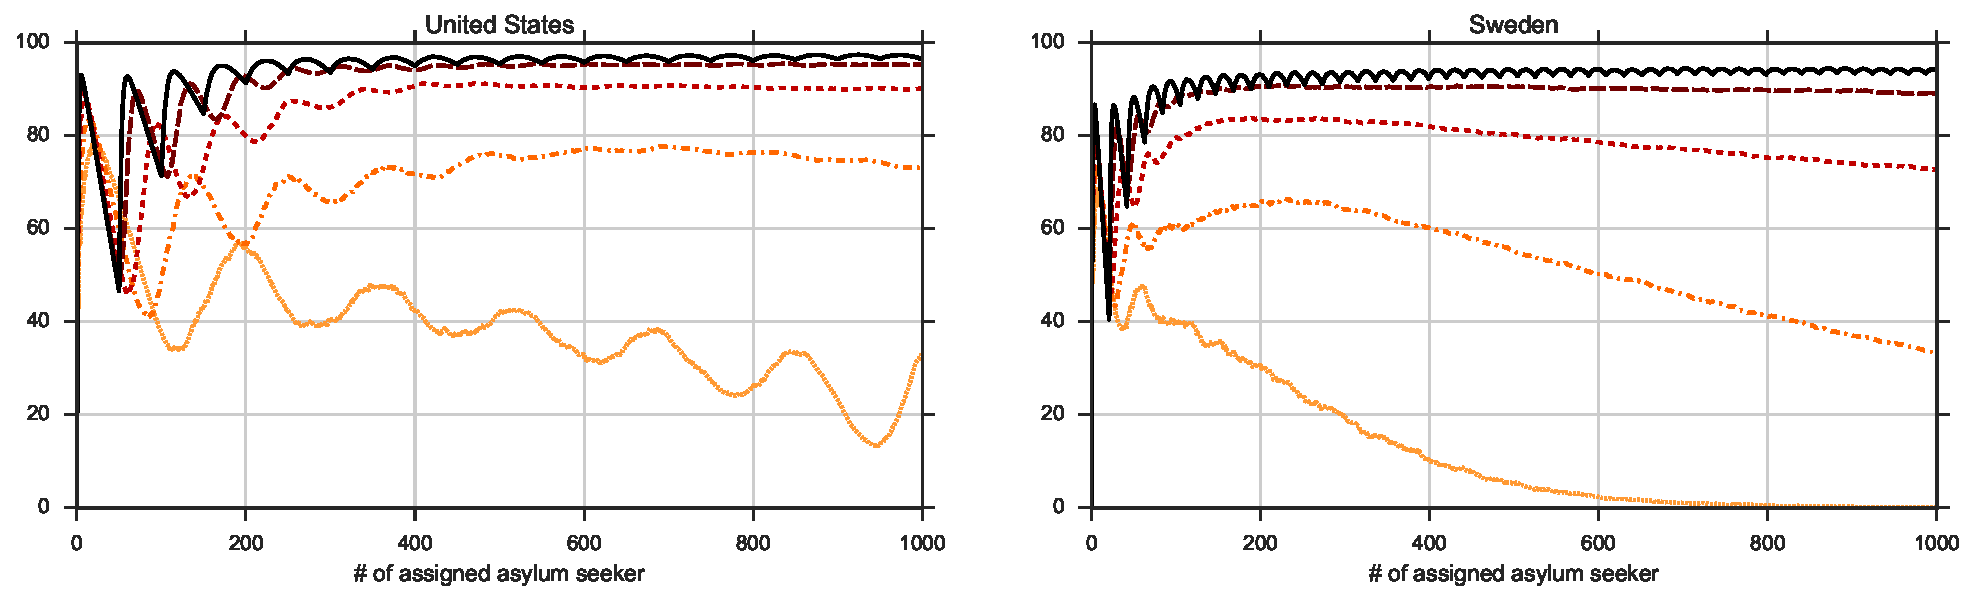
\includegraphics[width=\linewidth]{figs/misclassification/double_envy0_new.pdf}}
	\vspace{-0.7em}
	\subfloat[Percentage of localities envying some locality by at least five asylum seekers \label{SUBFIG-misclassification_fair1}]{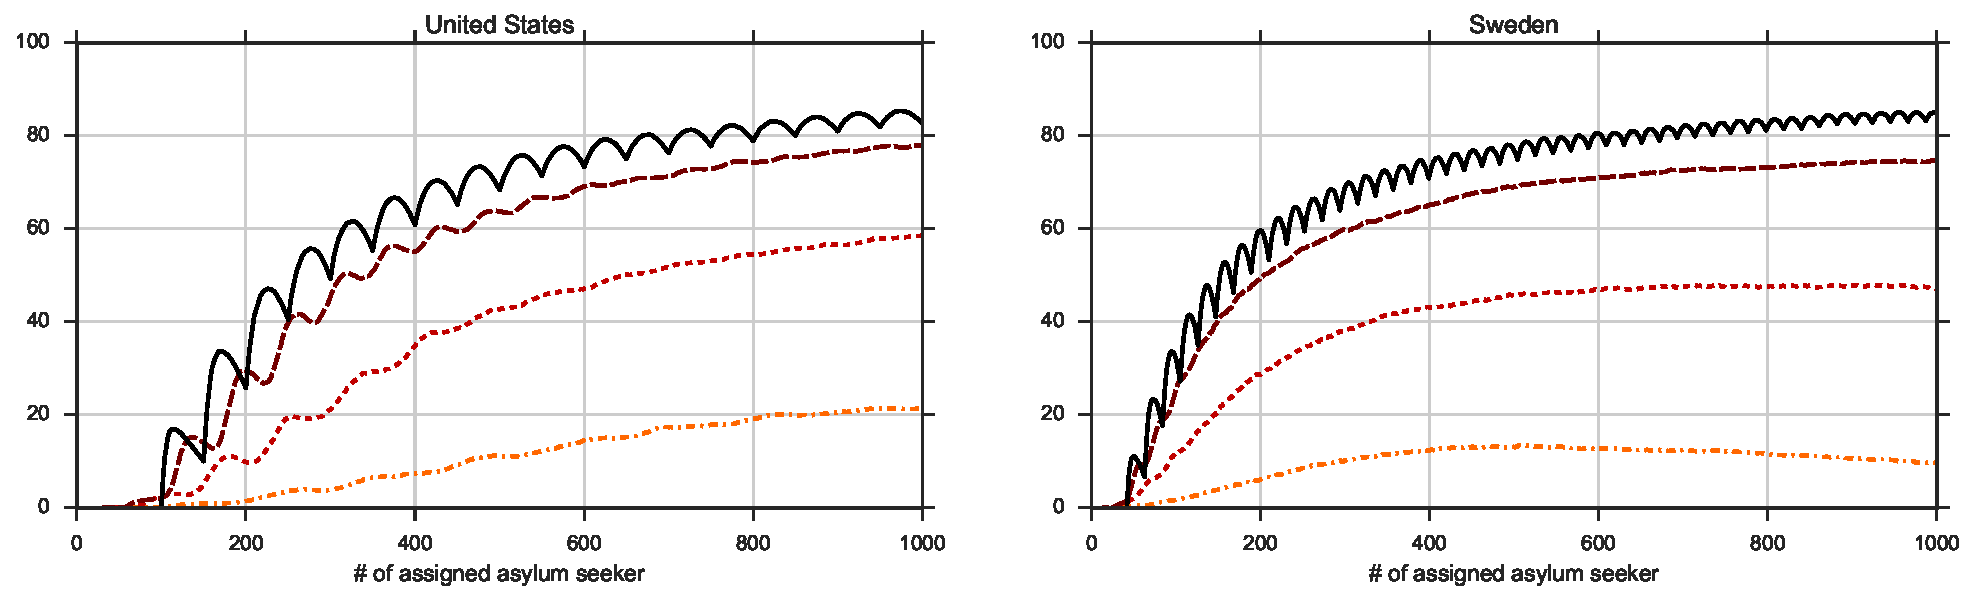
\includegraphics[width=\linewidth]{figs/misclassification/double_envy1_new.pdf}}
	\vspace{-0.7em}
	\subfloat[Percentage of mismatched acceptable asylum seekers \label{SUBFIG-misclassification_effic}]{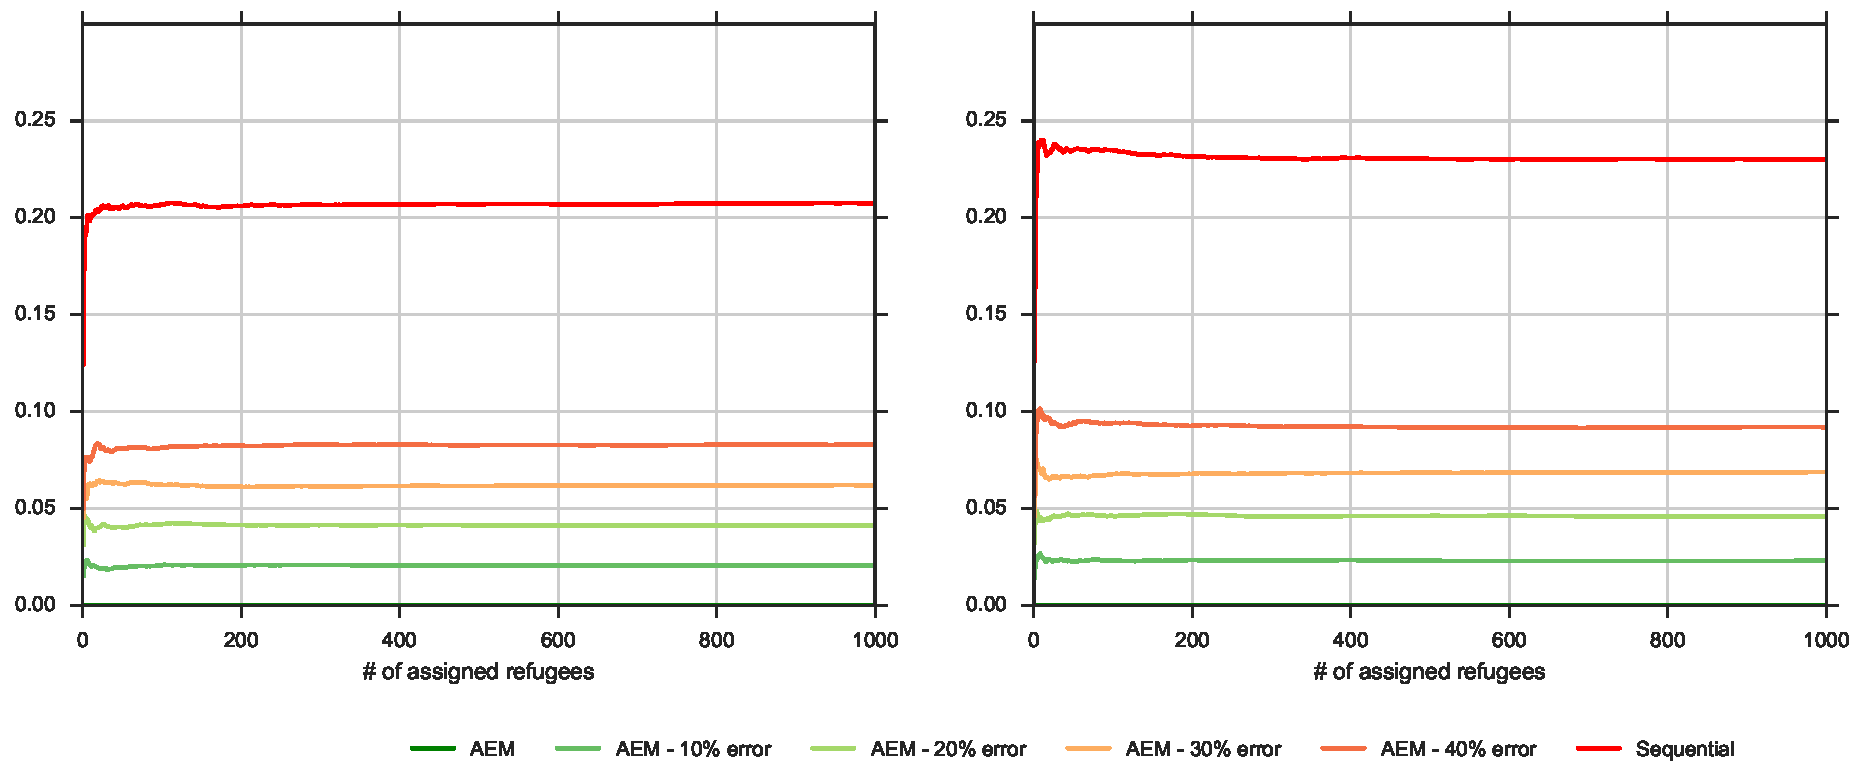
\includegraphics[width=\linewidth]{figs/misclassification/double_effic_new.pdf}}

	{\scriptsize \vspace{-1em}
	\begin{singlespace}
		{\sc Notes:} A thousand waves of asylum seekers of 1,000 asylum seekers each is simulated, distributed across 51 locations in the United States and the 21 Swedish regional entities (l{\"a}n). The measures of efficiency loss and envy are computed at each matching, comparing the performance of the proposed mechanism (with increasing degrees of misclassification error) with that of the na\"{i}ve sequential matching mechanism. The flows of asylum seekers are calibrated to match the numbers reported by \cite{bib:BansakEtAl} for the United States ($\overline{D}$: 34 percent; $\underline{D}$: 39 percent) and average 2016 employment outcomes of the 2013 asylum seeker wave in Sweden ($\overline{D}$: 28 percent; $\underline{D}$: 45 percent).
	\end{singlespace}
	 }
\end{figure}

Figure \ref{FIG-miclassification} compares the performance of the proposed mechanism (AEM) with increasing degrees of misclassification error in the locality-specific partitions with that of the na\"{i}ve sequential matching mechanism, in terms of both envy and efficiency loss. The proportion of localities in the sample envying some locality by at least one and at least five asylum seekers are used as measures of envy. If the locality-specific partitions are correct, Theorem \ref{THEOREM:envy_efficiency} shows that the proposed mechanism guarantees that envy is bounded by a single asylum seeker. Remarkably, Panel \ref{SUBFIG-misclassification_fair0} shows that the share of localities envying another locality by at least one asylum seeker decreases with the number of asylum seekers per locality, and converges towards zero. Even with misclassification error, Panels \ref{SUBFIG-misclassification_fair0} and \ref{SUBFIG-misclassification_fair1} in Figure \ref{FIG-miclassification} show that the proposed matching mechanism always outperforms the na\"{i}ve sequential matching mechanism in terms of envy. With the 24 percent misclassification error of \cite{bib:BansakEtAl}, in the Swedish case the proposed mechanism guarantees already after 1,000 arrivals a decrease of 23 percent in the share of envying municipalities, and of 45 percent in the share of envying municipalities by more than five asylum seekers (here it should be noted that there were around 25,000 asylum seekers in Sweden in 2016 and 2017).\footnote{The corresponding numbers for the US case are 7 and 30 percent respectively. The difference is primarily due to the higher number of localities in the US, causing envy measures with misclassification error to decrease more slowly. A replication of these measures for different combinations of $\overline{D}$ and $\underline{D}$ proportions for 21 localities appears in Appendix B.}

Efficiency loss is measured as the share of asylum seekers that, while acceptable for some localities, end up in a locality that considers them unacceptable. This measure reflects the preferences of asylum seekers of achieving the best possible outcomes for their future, and is in a Pareto efficient matching always equal to zero. Even with misclassification error, the proposed mechanism produces strong efficiency gains with respect to the na\"{i}ve sequential matching mechanism. With the 24 percent misclassification error of \cite{bib:BansakEtAl}, the proposed mechanism decreases the share of mismatched acceptable asylum seekers by around 50 percent.

\subsection{Choice of Quotas}\label{SEC:quotas}
The presence of heterogeneous quotas across localities introduces a further seasonality-related concern. For example, in Sweden each locality has the obligation by law of reserving housing units for asylum seekers \citep[Swedish Law,][]{SFS2016}. Yearly quotas coupled with the proposed mechanism will lead smaller localities to fill up all their housing obligation in a few months, and thus will be obliged to provide housing units only at a given time of the year. Larger localities will instead have to provide housing throughout the year. A solution to this disparity would be splitting yearly quotas in, e.g., trimester quotas, and dynamically match asylum seekers within each trimester. This section shows that such strategy is feasible and, as with random flows of asylum seekers, the performance of the proposed mechanism does not suffer from partitioning quotas across shorter time periods, and can actually improve for small enough misclassification error in the partition.

A thousand random flows of asylum seekers is simulated and calibrated as in Figure \ref{FIG-miclassification} for Sweden using the 2017 quotas.\footnote{These quotas are available at the website of the Swedish Migration Board (\texttt{www.migrationsverket.se}).} For each flow of asylum seekers, the quotas are splitted up at yearly, semestral, trimestral and monthly intervals.\footnote{In 2017, the sum of all quotas was 23,600. For simplicity, each yearly regional quota is rounded to a number divisible by 12, and thus flows of 23,568 asylum seekers are considered.} At each interval, the matching mechanism restarts either blindly (i.e., resetting the aggregated envy to at zero at the start of the considered period) or by initiating the mechanism in every subperiod after the first with the envy matrix calculated at the end of the previos period for all localities, including those which filled their quotas early in the sub-period. Therefore, even with no misclassification error in the partition, it's possible that localities which filled their quotas early in the sub-period envy (or are envied by) others by more than one asylum seeker at the beginning of subsequent sub-periods. The process of transferring envy measures across periods is referred to as envy legacy. The measures of envy and efficiency loss are then compared at the end of the year, when the flow of asylum seekers has been completely assigned. All results are benchmarked against those obtained through the na\"{i}ve sequential matching mechanism.

\begin{table}
\caption{ Performance of the assignment algorithm if quotas are split over multiple sub-periods}
\label{TABLE:quotas}
\makebox[\textwidth]{
	\scriptsize
	\begin{tabularx}{\linewidth}{lYYYYYYYY}
		\toprule\toprule
		& \multicolumn{4}{c}{Percentage of mismatched acceptable asylum seekers}
		& \multicolumn{4}{c}{Number of localities envying some locality} \\
		&&&&& \multicolumn{4}{c}{by at least one asylum seeker} \\
		\cmidrule(lr){2-5}\cmidrule(lr){6-9}
		 & Year & Semester & Trimester & Month & Year & Semester & Trimester & Month  \\
		\midrule
		\input{tabs/quotas_seq_0.txt} \\
		\input{tabs/quotas_aem_0.txt} \\
		\input{tabs/quotas_aem_legacy_0.txt}
		\bottomrule
	\end{tabularx}
	}
	{\scriptsize \vspace{0.1em}
	\begin{singlespace}
		{\sc Notes:} A thousand waves of 23,568 asylum seekers each is simulated, distributed across 21 Swedish regional entities (l\"{a}n) according to 2017 Swedish regional quotas. The table reports the average, standard deviation (in parentheses) and median (in brackets) of fairness and efficiency loss measures calculated after the assignment of the 23,568th asylum seeker for (i) the proposed mechanism restarted blindly, (ii) the proposed mechanism allowing for dynamic legacies in envy across sub-periods, and (iii) the na\"{i}ve sequential matching mechanism. Because the number of localities is constant, the table reports the number instead of the share of envying localities as fairness loss measure. Flows of asylum seekers are calibrated to match average 2016 employment outcomes of the 2013 asylum seeker wave in Sweden ($\overline{D}$: 28 percent; $\underline{D}$: 45 percent). Autocorrelation of locality preferences is allowed for each asylum seeker.
	\end{singlespace}
	 }
	\end{table}

This exercise reveals three relevant properties of the proposed order mechanism when constrained by heterogeneous quotas. Table \ref{TABLE:quotas} reports measures of efficiency and fairness loss computed at the end of the assignement year for each of the simulated asylum seeker flows across all localities, including those dropping out of the mechanism once their quota was filled. First, while the proposed mechanism can produce efficiency and fairness losses due to unequally sized quotas, it still strongly outperforms the standard na\"{i}ve sequential matching mechanism. Second, with random refugee flows, partitioning the quotas across subperiods and restarting the mechanism each time with zero envy across localities does not affect its performance. Third, allowing for envy matrices to be transferred across subperiods can improve fairness at a small efficiency loss.

While this last property emerges in this particular manner in the specific Swedish situation, examining the sources of thise trade-off delivers an intuitive understanding of the implicit trade-off between efficiency and fairness created by heterogeneous quotas. The largest regional entity in Sweden receives alone 30\% of all asylum seekers in a given year, with the second and third largest locality receiving 16\% and 12\% respectively. This inequality implies that the largest localities will tbe the last to fill their quotas, and thus a mechanism satisfying rotation will assign the last thousands asylum seekers in a subperiod always to those localities, independently on their type. Because the calibrations of the asylum seeker flows imply that a random refugee is more likely to be unacceptable than acceptable for a given locality, it follows that the largest regional entities will accumulate a lot of envy towards the smaller localities.

With yearly quotas, the largest entity envies some other smaller locality in every simulation, and the second or third largest 24\% of the times. By partitioning yearly quotas into smaller intervals and allowing for envy legacy across subperiods, municipalities that have accumulated lots on envy in the previous subperiods are more likely to be at the first places in the priority order. Therefore, they receive relatively more acceptable asylum seekers in the following period, and fill their quotas slightly faster. As a consequence, the second and third largest locality never envy any other locality anymore. However, as they fill their quotas earlier, a longer tail flow of asylum seekers can only be assigned to the largest locality at the end of the period, thereby slightly reducing efficiency. 

This process highlights that order mechanism that satisfies rotation with heterogenous locality-asylum seeker synergies performs better the longer a large enough amount of localities remains in the market. More available localities imply a higher likelihood that one of them finds an asylum seeker acceptable, thereby---by exploiting an informed assignment mechanism---simultaneously improving efficiency and fairness.

\subsection{The Envy Bounded by One Conjecture}
As discussed in Section \ref{SEC:Structure_Mechanisms}, we conjecture that envy is always bounded by a single acceptable asylum seeker \emph{and} a single unacceptable asylum seeker whenever the matching is selected by an order mechanism that satisfies rotation. To provide some empirical evidence for this conjecture, 5,000 waves of 1,000 seekers each are simulated, distributed across 20 localities, assuming that the characteristics of the refugee flow are random. This simulation gives a total of 100 million envy measures by locality. Envy measures are split across envy on acceptable asylum seekers (another municipality has more asylum seekers considered acceptable) and envy on unacceptable asylum seekers (another municipality has less asylum seekers considered unacceptable). 

\begin{table}[h]
\caption{Simulation results for the conjecture that envy is bounded by one in acceptable and unacceptable asylum seekers.}
\label{TABLE:conjecture_1}
\makebox[\textwidth]{
	\scriptsize
	\begin{tabularx}{\linewidth}{lYYYYYYYY}
		\toprule\toprule
		 & p10 & p50 & p90 & max & p10 & p50 & p90 & max  \\
		\midrule
		Assigned asylum seekers & \multicolumn{4}{c}{\emph{Acceptable asylum seekers}}
		& \multicolumn{4}{c}{\emph{Unacceptable asylum seekers}} \\
		\cmidrule(lr){2-5}\cmidrule(lr){6-9}
		\input{tabs/simres.txt}
		\bottomrule
	\end{tabularx}
}
{\scriptsize \vspace{0.1em}
	\begin{singlespace}
		{\sc Notes:} Five thousand waves of one thousand asylum seekers each is simulated, distributed across 20 regional entities, delivering a total of 100 million locality-specific meximum envy measures (the highest envy towards any of the remaining 19 localities). The table reports the maximum, $90^{th}$, $50^{th}$, and $10^{th}$ percentile of maximum envy at specific intervals of asylum seeker arrival. Envy on acceptable asylum seekers is separated from envy on unascceptable asylum seeker. The characteristics of the refugee flow (proportions of $\overline{D}$ and $\underline{D}$ asylum seeker and autocorrelation of preferences across municipalities) is randomized for each asylum seeker flow. 
	\end{singlespace}
	 }
	\end{table}

Table \ref{TABLE:conjecture_1} shows the 10th, 50th and the 90th percentile of observed maximum envy across these 100 million observations, arranged by three intervals of number of assigned asylum seeker in the flow (1--100, 101--500, and 501--1,000). As can be seen from the table, the conjecture is not violated a single time. Moreover, the low percentiles of envy measures are decreasing with the number of arrivals, implying that the likelihood of a locality to be truly unenvious increases with the number of assigned asylum seekers.


\section{Conclusions}\label{SEC:conclusions}
This paper has investigated dynamic refugee matching as a market design application. A specific matching mechanism was proposed and it has been demonstrated that any matching selected by the proposed mechanism is Pareto efficient and satisfies envy bounded by a single asylum seeker. This theoretical finding hinges on the assumption that there is no misclassification error. For example, \cite{bib:BansakEtAl} report 24 percent misclassification error for their preferred refugee assignment models estimated on US data. However, even with a 24 percent misclassification error, the proposed mechanism (i) decreases the share of mismatched acceptable asylum seekers by around 50 percent and (ii) reduces envy by between 7 and 45 percent.

This paper does not empirically estimate prediction functions, as we currently do not have access to the necessary data. By exploiting refugee data from the United States and Switzerland, \cite{bib:BansakEtAl} estimate locality-specific partitions by a machine learning algorithm, allowing for locality-specific synergies with heterogeneous refugees. Because their algorithm focuses on minimizing prediction error rather than uncovering structural parameters determining labor market success \citep{bib:MullainathanSpiess}, machine learning is a particularly appropriate tool in this context. Such an unstructured approach highlights the low external validity of the estimated prediction function, which therefore needs to be re-estimated and re-calibrated in different scenarios and as new data becomes available. The necessity to update the prediction function has the benefit of alleviating the problem of displacement and general equilibrium effects due to the field implementation of mechanisms as the one proposed in this paper \citep{bib:CreponEtAl}. If the labor demand for asylum seekers is very inelastic, then even an efficient assignment does not guarantee employment for asylum seekers predicted as acceptable. In practice, this mismatch would increase prediction error in our predictions. However, re-estimating the prediction function with updated data would capture these effects and return a better predicted ``demand matrix'' in a later stage.

A more theoretical remark is that the proposed mechanism assumes that asylum seekers arrive one-by-one. This means that the current form of the mechanism does not take families of asylum seekers into account \citep[see, e.g.,][for a mechanism that keeps families intact in house allocation problems with asylum seekers]{bib:AnderssonEhlers}. To also account for families, each asylum seeker can be described to be of a specific size representing the number of family members and some (limited) flexibility in the quotas must be introduced. In this case, envy cannot be guaranteed to be bounded by a single asylum seeker but is instead bounded by the maximal family size in the sequence.

Finally, this paper has abstracted from issues related to manipulability. It is  well-established in the mechanism design literature that agents (localities in this paper) often cannot be prevented from manipulating mechanisms in their advantage by misrepresenting preferences. In the framework investigated in this paper, this means that localities may gain by classifying an acceptable asylum seeker as unacceptable or vice versa. To analyze this type of strategic behavior, some notion of dynamic (non-)manipulability needs to be introduced. Such analysis is beyond the scope of this paper. Also, because the preferences exploited in this paper are derived from estimation and not first-party reports, manipulability is unlikely to constitute a major problem in the considered dynamic refugee matching problem.


\bibliographystyle{chicago}
\bibliography{ref}
\newpage

\section*{Appendix A: Proofs}
This Appendix contains the proofs of all results in the paper.

\medskip

\noindent\textbf{Proof of Theorem \ref{THEOREM:envy_efficiency}.} To prove part (i), suppose that envy not is bounded by a single asylum seeker at matching $x(k)$. This means that there are two localities in $M(k)$, say $m$ and $m^\prime$, and two integers, say $k^0$ and $k^1$ (where $0<k^0<k^1\leq k$), such that:
\begin{itemize}
\item[(I)] locality $m$ is indifferent between bundles $x_{m}(k^0-1)$ and $x_{m^\prime}(k^0-1)$,
\item[(II)] locality $m$ envies locality $m^\prime$ by exactly one asylum seeker at matching $x(k^0)$,
\item[(III)] locality $m$ envies locality $m^\prime$ by exactly two asylum seekers at matching $x(k^1)$.
\end{itemize}
\noindent Let $k^0$ and $k^1$ be the largest and the smallest integers, respectively, satisfying conditions (I)--(III), and consider the subsequence $(s(k^0),\ldots,s(k^1))$ of the sequence $s$. Because the integers $k^0$ and $k^1$ are chosen in the above way, locality $m$ is not matched to any asylum seeker in the subsequence $(s(k^0+1),\ldots,s(k^1-1))$, and
locality $m^\prime$ is not matched to any non-demanded asylum seeker or any asylum seeker that is acceptable for locality $m$ in the subsequence $(s(k^0+1),\ldots,s(k^1-1))$. Hence, there four reasons to why conditions (I)--(III) hold:
\begin{itemize}
\item[(a)] Asylum seekers $s(k^0)$ and $s(k^1)$ are acceptable to locality $m$ but both $s(k^0)$ and $s(k^1)$ are matched to locality $m^\prime$,
\item[(b)] asylum seeker $s(k^0)$ is non-demanded but matched to locality $m$ and asylum seeker $s(k^1)$ is acceptable to locality $m$ but matched to locality $m^\prime$,
\item[(c)] asylum seeker $s(k^0)$ is acceptable to locality $m$ but matched to locality $m^\prime$ and asylum seeker $s(k^1)$ is non-demanded but matched to locality $m$,
\item[(d)] asylum seekers $s(k^0)$ and $s(k^1)$ are non-demanded but both are matched to locality $m$.
\end{itemize}
\noindent It is only proved that cases (a) and (b) cannot occur as the corresponding proofs of cases (c) and (d) are almost identical.

To prove that (a) cannot occur, note that asylum seeker $s(k^0)$ is acceptable for both $m$ and $m^\prime$. Hence, by rotation of $(\pi,\sigma)$, it follows that locality $m^\prime$ has a higher position than locality $m$ in $\pi(k^0)$ and the lowest position in $\pi(k^0+1)$. Because asylum seeker $s(k^1)$ is matched to locality $m^\prime$, it must also be the case that locality $m^\prime$ has a higher position than locality $m$ in $\pi(k^1)$. The latter can, however, not occur. To see this, recall first that locality $m$ is not matched to any asylum seeker in the subsequence $(s(k^0),\ldots,s(k^1))$.
Similarly, $m^\prime$ is not matched to any asylum seeker in the subsequence $(s(k^0+1),\ldots,s(k^1-1))$. Hence, by rotation of $(\pi,\sigma)$, the relative positions among $m$ and $m^\prime$ do not change for the priority orders $\pi(k^0+1),\ldots,\pi(k^1)$, which is a contradiction to $m^\prime$ being matched to the demanded asylum seeker $s(k^1)$.

To prove that (b) cannot occur, recall that asylum seeker $s(k^0)$ is non-demanded and that locality $m$ envies locality $m^\prime$ at matching $x(k^0)$. Hence, by rotation of $(\pi,\sigma)$, locality $m$ has a higher position than locality $m^\prime$ in $\pi(k^0+1)$. Because the overdemanded asylum seeker $s(k^1)$ is matched to locality $m^\prime$, it must be the case that locality $m^\prime$ has a higher position than locality $m$ in $\pi(k^1)$.
The latter can, however, not occur. To see this, recall first that locality $m$ is not matched to any asylum seeker in the subsequence $(s(k^0),\ldots,s(k^1))$. Similarly, $m^\prime$ is not matched to any asylum seeker in the subsequence $(s(k^0+1),\ldots,s(k^1-1))$. Hence, by rotation of $(\pi,\sigma)$, the relative positions among $m$ and $m^\prime$ do not change for the priority orders $\pi(k^0+1),\ldots,\pi(k^1)$, which is a contradiction to $m^\prime$ being matched to the demanded asylum seeker $s(k^1)$.

To prove part (ii), suppose that $x(k)$ is not Pareto efficient. Consider the localities in the set $M(k)$ and the asylum seekers in the set $A(k)$. Because $x(k)$ is not Pareto efficient, by assumption, there exists a matching $x^\prime(k)$ where the quotas are respected for all localities in $M(k)$, $x_m^\prime(k)R_m(k) x_m(k)$ for all $m\in M(k)$, and $x_m^\prime(k)P_m(k) x_m(k)$ for some $m\in M(k)$. The latter conditions imply that:
\begin{equation}
\sum_{j\in M(k)}\left(|A_j^+(x_j^\prime(k))|-|A_j^-(x_j^\prime(k))|\right)>\sum_{j\in M(k)}\left(|A_j^+({x_j}(k))|-|A_j^-({x_j}(k))|\right).\label{EQ:not_efficient_A}
\end{equation}
\noindent Note next that a locality in $M(k)$ can only be matched to an unacceptable asylum seeker if the asylum seeker also is unacceptable for all other localities in $M(k)$. This follows since $\varphi$ is an order mechanism. But this also means that $\sum_{j\in M(k)}|A_j^-(x_j^\prime(k))|=\sum_{j\in M(k)}|A_j^-({x_j}(k))|$. Consequently, condition (\ref{EQ:not_efficient_A}) reduces to:
\begin{equation}
\sum_{j\in M(k)}|A_j^+(x_j^\prime(k))|>\sum_{j\in M(k)}|A_j^+({x_j}(k))|,\label{EQ:not_efficient_B}
\end{equation}
\noindent i.e., that the total number of acceptable asylum seekers matched to the localities in $M(k)$ is greater at matching $x^\prime(k)$ than at matching $x(k)$. But this is not possible since all asylum seekers in $A(k)$ are matched to some locality in $M(k)$ which finds them acceptable by construction of the order mechanism $\varphi$. Hence, $x(k)$ must be Pareto efficient. \hfill $\square$

\medskip

\noindent\textbf{Proof of Corollary \ref{COROLLARY:envy}.} Because matching $x(k)$ is selected by $\varphi$, it follows from Theorem \ref{THEOREM:envy_efficiency} that envy for locality $m$ towards locality $m^\prime$ is bounded by a single asylum seeker, i.e., that:
\begin{equation}
|A_m^+(x_m(k))|-|A_m^-(x_m(k))|+1\geq |A_m^+(x_{m^\prime}(k))|-|A_m^-(x_{m^\prime}(k))|.\label{EQ:COR_1}
\end{equation}
\noindent To obtain a contradiction, suppose now that the statement is not true. Then:
\begin{eqnarray}
&& |A_m^+(x_{m^\prime}(k))|>|A_m^+(x_m(k))|,\label{EQ:COR_2} \\
&& |A_m^-(x_m(k))|>|A_m^-(x_{m^\prime}(k))|.\label{EQ:COR_3}
\end{eqnarray}
\noindent Inequality (\ref{EQ:COR_2}) implies $|A_m^+(x_{m^\prime}(k))|-1\geq |A_m^+(x_m(k))|$. This condition together with inequality (\ref{EQ:COR_1}) implies $|A_m^-(x_{m^\prime}(k))|\geq |A_m^-(x_m(k))|$. But the latter inequality contradicts inequality (\ref{EQ:COR_3}).~\hfill$\square$

\medskip

\noindent\textbf{Proof of Theorem \ref{TH:structures}.} It is only proved that locality $m$ does not envy any locality with a higher position in $\pi(k+1)$ since the second part of the theorem is based on symmetrical arguments. The result is proved by induction. It is first demonstrated that the result is true for $\pi(2)$. Three cases must be considered:

\begin{itemize}

\item[(1.a)] \emph{Asylum seeker $s(1)$ is non-demanded.} Because $s(1)$ is non-demanded, no locality in $m(1)$ will envy the locality which is matched to $s(1)$ and the locality which is matched to $s(1)$ will envy all localities in $M(1)$. Because $(\pi,\sigma)$ satisfies rotation, the locality that is matched to $s(1)$ will have the highest position in $\pi(2)$. These arguments show that no locality in $M(1)$ envies any locality with a higher position in $\pi(2)$.

\item[(1.b)] \emph{Asylum seeker $s(1)$ is demanded.} In this case, $s(1)$ is matched to the only locality finding $s(1)$ acceptable, and no locality will envy this locality. Similarly, the locality which is matched to $s(1)$ will not envy any other locality since $s(1)$ is acceptable. Because $(\pi,\sigma)$ satisfies rotation, it follows that $\pi(1)=\pi(2)$, and, consequently, no locality in $M(1)$ envies any locality with a higher priority in $\pi(2)$.

\item[(1.c)] \emph{Asylum seeker $s(1)$ is overdemanded.} In this case, asylum seeker $s(1)$ is matched to the locality in $M(1)$ with the highest position in $\pi(1)$ which finds asylum seeker $s(1)$ acceptable. This locality will be envied by all localities finding $s(1)$ acceptable, and the locality which is matched to $s(1)$ will not envy any locality in $M(1)$. Because $(\pi,\sigma)$ satisfies rotation, the locality which is matched to $s(1)$ will have the lowest priority in $\pi(2)$. These arguments show that no locality in $M(1)$ envies any locality with a higher position in $\pi(2)$.
\end{itemize}

\noindent From the above arguments, it is concluded that the statement is true for $\pi(2)$. Consider now the induction hypothesis that the result holds for $\pi(k)$ for an arbitrary $k\in \{2,\ldots,n-1\}$. Given this assumption, it remains to show that the result is true for $\pi(k)$. Again, three cases must be considered:

\begin{itemize}
\item[($k$.a)] \emph{Asylum seeker $s(k)$ is non-demanded.} Because asylum seeker $s(k)$ is not acceptable to any locality in $M(k)$ and because envy is bounded by a single asylum seeker at matching $x(k-1)$ by Theorem \ref{THEOREM:envy_efficiency}, no locality in $M(k)$ will envy the locality which is matched to $s(k)$ at matching $x(k)$. Because $(\pi,\sigma)$ satisfies rotation, the locality which is matched to $s(k)$ will have a higher priority in $\pi(k+1)$ than all localities which the locality envies at matching $x(k)$. These arguments show that no locality in $M(k)$ envies any locality with a higher position in $\pi(k+1)$.

\item[($k$.b)] \emph{Asylum seeker $s(k)$ is demanded.} In this case, asylum seeker $s(k)$ is matched to the only locality which finds $s(k)$ acceptable. Because $(\pi,\sigma)$ satisfies rotation, it follows that $\pi(k)=\pi(k+1)$. Consequently, the result holds for $\pi(k+1)$ since the result is true for $\pi(k)$ by the induction hypothesis.

\item[($k$.c)] \emph{Asylum seeker $s(k)$ is overdemanded.} In this case, asylum seeker $s(k)$ is matched to the locality in $M(k)$ with the highest position in $\pi(k)$ finding asylum seeker $s(k)$ acceptable. Because envy is bounded by a single asylum seeker at matching $x(k-1)$ by Theorem \ref{THEOREM:envy_efficiency}, the locality which is matched to the acceptable asylum seeker $s(k)$ will not envy any locality at matching $x(k)$. Then by rotation of $(\pi,\sigma)$, the locality which is matched to $s(k)$ will have the lowest position in $\pi(k+1)$. But then the result holds by the above arguments.
\end{itemize}

\noindent The above three cases, together with the result for $\pi(2)$ and the induction assumption, proves that locality $m$ does not envy any locality with a higher priority in $\pi(k)$. \hfill $\square$

\section*{Appendix B: Additional Simulation Results}

This Appendix collects additional simulation results and further checks on the robustness of the performance of the order mechanism as the characteristics of refugee flows vary. Tables \ref{TABLE:big_appendix_1} and \ref{TABLE:big_appendix_2} report the expected percentage improvement in measures of fairness and efficiency granted by the proposed mechanism over the na\"{i}ve sequential matching mechanism for varying combinations of the proportion of non-demanded ($\underline{D}$) and always demanded ($\overline{D}$) asylum seekers in simulated arrival flows. For each combination of parameters, 1,000 refugee flows of 1,000 asylum seekers each are simulated and allocated to 21 localities. Each table row reports the average percentage difference across these simulated flows after the mechanism allocated the last refugee in the flow. All simulations allow for correlation of locality preferences for each asylum seeker.

The tables show that the relative improvement in fairness with respect to the na\"{i}ve sequential matching mechanism is larger when misclassification error is lower and the proportion of asylum seekers in the set $D$ is higher. The relative improvement in efficiency depends solely on the extent of misclassification error, and always ranges between 100 and 0 percent. The only exceptions consist in the situations in which all asylum seekers are either all in the set $\underline{D}$ or all in the set $\overline{D}$, where both assignment strategies produce Pareto efficient and fair allocations. The na\"{i}ve sequential matching mechanism always produces a Pareto efficient (but not necessarily fair) allocation if no asylum seekers of type $D$ exist.

Figure \ref{FIG-bad_assignments} shows that the na\"{i}ve sequential matching mechanism outperforms a truly random mechanism in terms of fairness. This result is due to the fact that the sequential assignment guarantees at least that the difference in the number of asylum seekers across localities is bounded by one.

Finally, Figure \ref{FIG:conjecture_1} provides evidence for the conjecture that envy is bounded by a single acceptable asylum seeker \emph{and} a single unacceptable asylum seeker.

\begin{table}
\caption{Simulated relative reduction in efficiency and envy measures with the proposed algorithm, by misclassification error in locality partitions, percentage of asylum seekers in set $\underline{D}$ and percentage of asylum seekers in set $\overline{D}$ in the simulated flows (I).}
\label{TABLE:big_appendix_1}
\makebox[\textwidth]{
	\scriptsize
	\begin{tabularx}{\linewidth}{lYYYYYYYYYY}
		\toprule\toprule
		& \multicolumn{5}{c}{\emph{Percentage decrease in the share of localities}} & \multicolumn{5}{c}{\emph{Percentage decrease in the share of}}\\
		& \multicolumn{5}{c}{\emph{envying some locality by at least one asylum seeker}} & \multicolumn{5}{c}{\emph{mismatched acceptable asylum seekers}}\\
		\cmidrule(lr){2-6}\cmidrule(lr){7-11}
		Miscl. error: & 0\% & 10\% & 25\% & 40\% & 50\%   & 0\% & 10\% & 25\% & 40\% & 50\%  \\
		\midrule
		$\%\underline{D}$ in flow & \multicolumn{10}{c}{$\%\overline{D}$ in flow: $0.00$} \\
		\cmidrule(lr){2-11}
		\input {tabs/errtable_overD0.txt} \\
		$\%\underline{D}$ in flow & \multicolumn{10}{c}{$\%\overline{D}$ in flow: $10.00$} \\
		\cmidrule(lr){2-11}
		\input {tabs/errtable_overD10.txt} \\
		$\%\underline{D}$ in flow & \multicolumn{10}{c}{$\%\overline{D}$ in flow: $20.00$} \\
		\cmidrule(lr){2-11}
		\input {tabs/errtable_overD20.txt} \\
		$\%\underline{D}$ in flow & \multicolumn{10}{c}{$\%\overline{D}$ in flow: $30.00$} \\
		\cmidrule(lr){2-11}
		\input {tabs/errtable_overD30.txt} \\
		\bottomrule
	\end{tabularx}
}
\end{table}

\begin{table}
\caption{Simulated relative reduction in efficiency and envy measures with the proposed algorithm, by misclassification error in locality partitions, percentage of asylum seekers in set $\underline{D}$ and percentage of asylum seekers in set $\overline{D}$ in the simulated flows (II).}
\label{TABLE:big_appendix_2}
\makebox[\textwidth]{
	\scriptsize
	\begin{tabularx}{\linewidth}{lYYYYYYYYYY}
		\toprule\toprule
		& \multicolumn{5}{c}{\emph{Percentage decrease in the share of localities}} & \multicolumn{5}{c}{\emph{Percentage decrease in the share of}}\\
		& \multicolumn{5}{c}{\emph{envying some locality by at least one asylum seeker}} & \multicolumn{5}{c}{\emph{mismatched acceptable asylum seekers}}\\
		\cmidrule(lr){2-6}\cmidrule(lr){7-11}
		Miscl. error: & 0\% & 10\% & 25\% & 40\% & 50\%   & 0\% & 10\% & 25\% & 40\% & 50\%  \\
		\midrule
		$\%\underline{D}$ in flow & \multicolumn{10}{c}{$\%\overline{D}$ in flow: $40.00$} \\
		\cmidrule(lr){2-11}
		\input {tabs/errtable_overD40.txt} \\
		$\%\underline{D}$ in flow & \multicolumn{10}{c}{$\%\overline{D}$ in flow: $50.00$} \\
		\cmidrule(lr){2-11}
		\input {tabs/errtable_overD50.txt} \\
		$\%\underline{D}$ in flow & \multicolumn{10}{c}{$\%\overline{D}$ in flow: $60.00$} \\
		\cmidrule(lr){2-11}
		\input {tabs/errtable_overD60.txt} \\
		$\%\underline{D}$ in flow & \multicolumn{10}{c}{$\%\overline{D}$ in flow: $70.00$} \\
		\cmidrule(lr){2-11}
		\input {tabs/errtable_overD70.txt} \\
		$\%\underline{D}$ in flow & \multicolumn{10}{c}{$\%\overline{D}$ in flow: $80.00$} \\
		\cmidrule(lr){2-11}
		\input {tabs/errtable_overD80.txt} \\
		$\%\underline{D}$ in flow & \multicolumn{10}{c}{$\%\overline{D}$ in flow: $90.00$} \\
		\cmidrule(lr){2-11}
		\input {tabs/errtable_overD90.txt}
		\bottomrule
	\end{tabularx}
}
\end{table}


\begin{center}
\begin{figure}
	\caption{Comparison of sequential and truly random assignments \label{FIG-bad_assignments}.}
	\begin{center}
	\subfloat[Percentage of localities envying some locality by at least one asylum seeker]{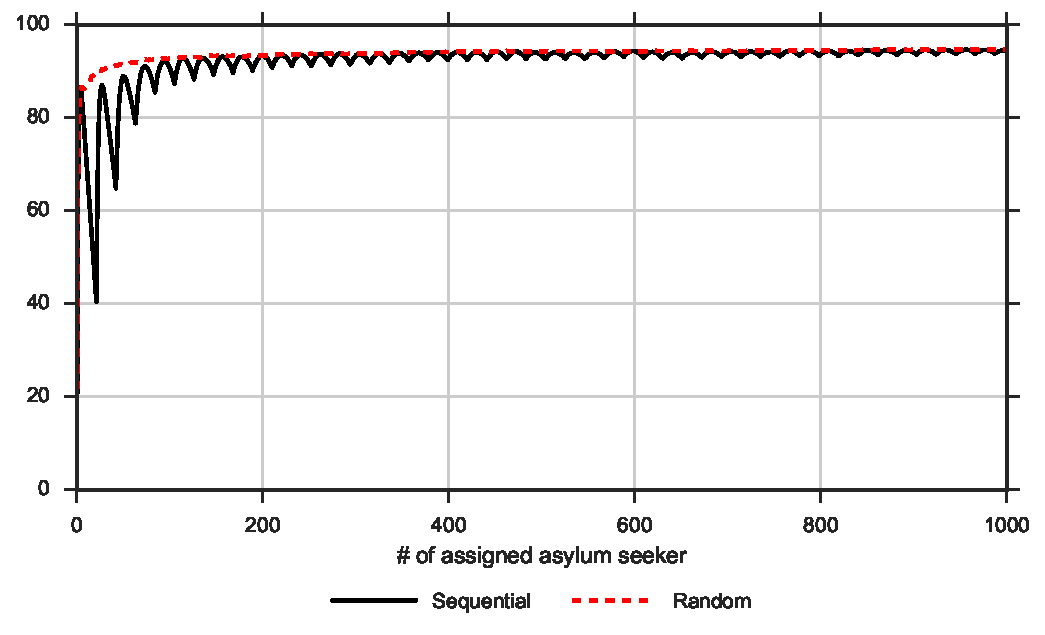
\includegraphics[width=0.5\linewidth]{figs/bad_assignments/single_envy0.pdf}}%

	\subfloat[Percentage of localities envying some locality by at least five asylum seeker]{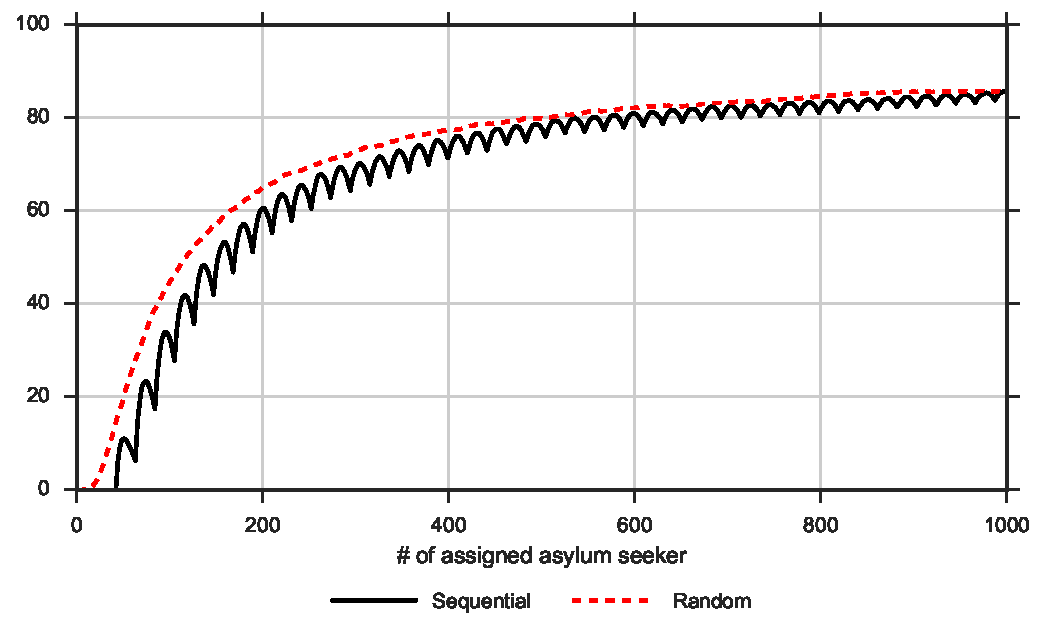
\includegraphics[width=0.5\linewidth]{figs/bad_assignments/single_envy1.pdf}}%

	\subfloat[Percentage of mismatched acceptable asylum seekers]{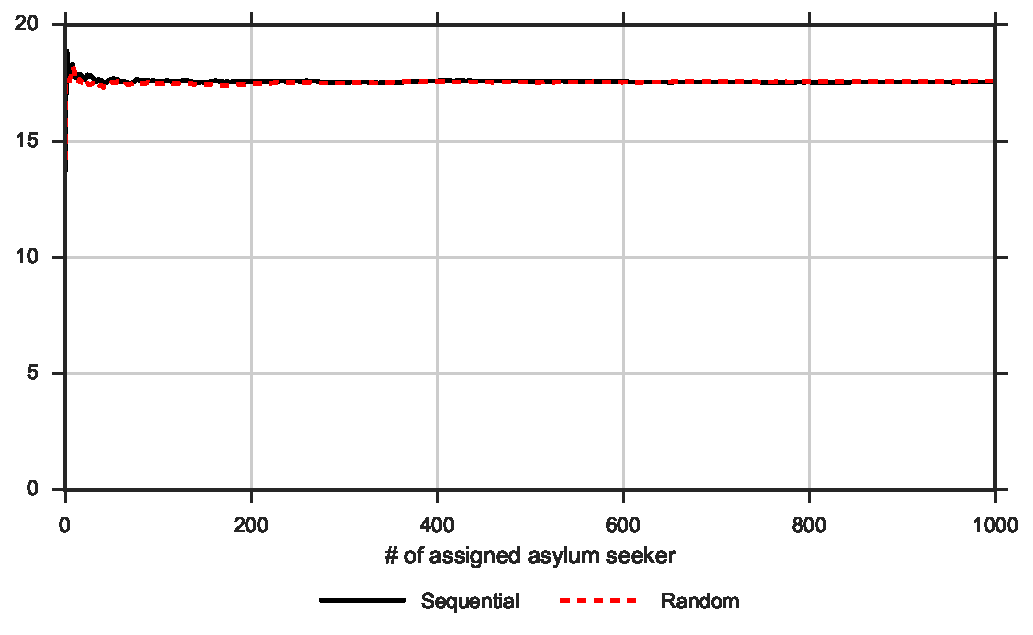
\includegraphics[width=0.5\linewidth]{figs/bad_assignments/single_effic.pdf}}
	\end{center}
		{\scriptsize \vspace{-1em}
	\begin{singlespace}
		{\sc Notes:} 1,000 waves of asylum seekers of 1,000 asylum seekers each is simulated, distributed across 21 Swedish regional entities (l{\"a}n). The measures of efficiency and envy is computed at each matching, comparing the performance of the na\"{i}ve sequential matching mechanism with that of the truly random assignment mechanism. The flows of asylum seekers are calibrated to match the average 2016 employment outcomes of the 2013 asylum seeker wave in Sweden ($\overline{D}$: 28 percent; $\underline{D}$: 45 percent).
	\end{singlespace}
	 }
\end{figure}
\end{center}

\begin{figure}
	\caption{Simulation for the conjecture that envy is bounded by one in acceptable and unacceptable asylum seekers.\label{FIG:conjecture_1}}
	\begin{center}
		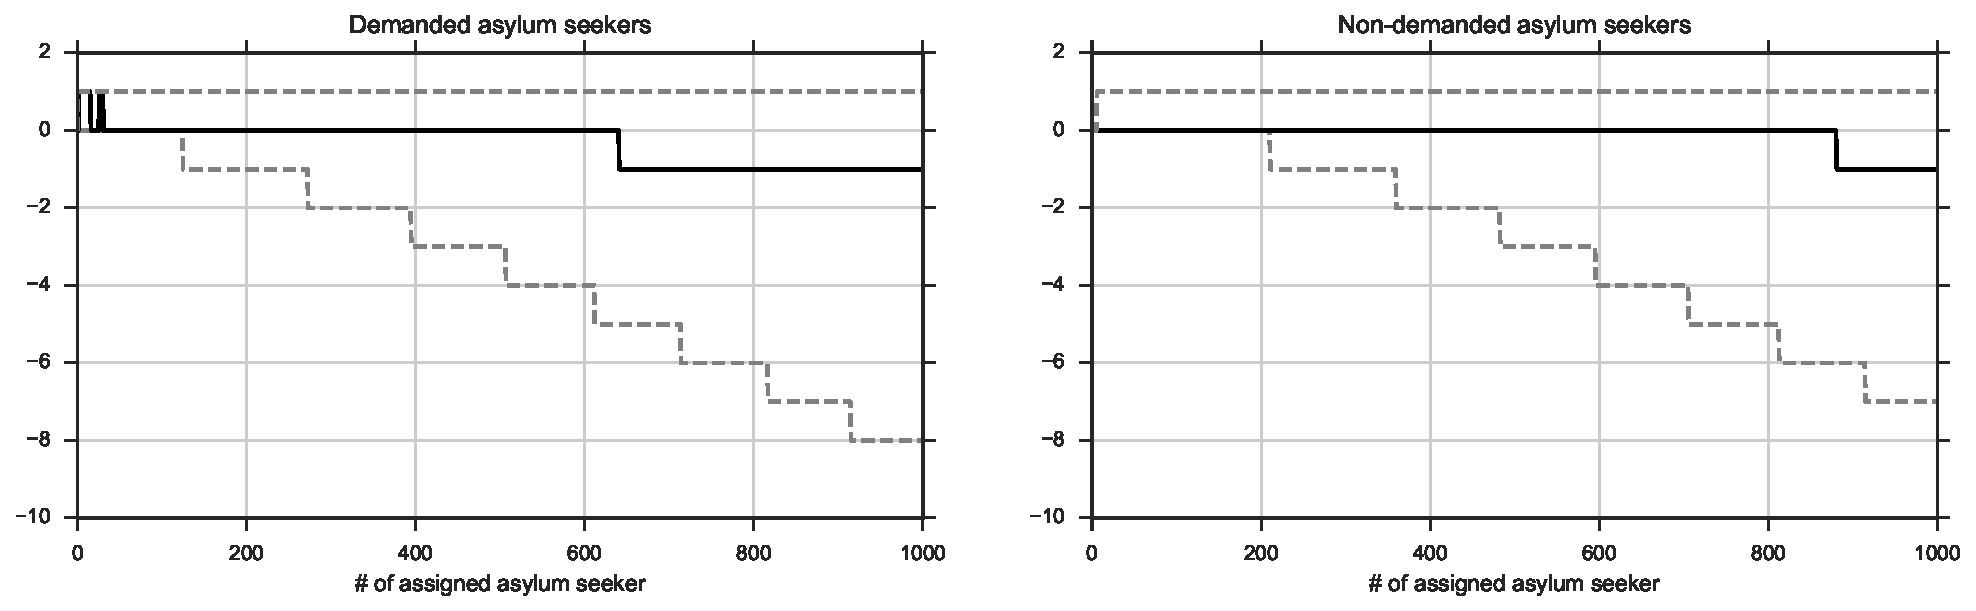
\includegraphics[width=\linewidth]{figs/conjecture/both.pdf}
	\end{center}
		{\scriptsize \vspace{-1em}
	\begin{singlespace}
		{\sc Notes:} 5,000 waves of 1,000 asylum seekers each is simulated, distributed across 20 localities. The characteristics of the refugee flow are random. This simulation gives us a total of 100 million maximum envy measures by locality (the maximum envy that each locality has towards any of the remaining 19 localities). Envy measures are split across envy on acceptable asylum seekers (another municipality has more asylum seekers considered acceptable) and envy on unacceptable asylum seekers (another municipality has less asylum seekers considered unacceptable). The figure plots the maximum, median and minimum observed maximum envy across these 100 million observations, arranged by number of assigned asylum seeker in the flow. The maximum measure never exceeds one for either acceptable and unacceptable asylum seekers, while the minimum of maximum envy decreases with the number of assigned asylum seekers.
	\end{singlespace}
	 }
\end{figure}

\end{document}
